% !TeX spellcheck = hu_HU
% !TeX encoding = UTF-8
% !TeX program = xelatex
% TODO Change language to en_GB (recommended) or en_US for English documents
\documentclass[11pt,a4paper,oneside]{report}             % Single-side
%\documentclass[11pt,a4paper,twoside,openright]{report}  % Duplex

% thanks to http://tex.stackexchange.com/a/47579/71109
\usepackage{ifxetex}
\usepackage{ifluatex}
\newif\ifxetexorluatex % a new conditional starts as false
\ifnum 0\ifxetex 1\fi\ifluatex 1\fi>0
   \xetexorluatextrue
\fi

\ifxetexorluatex
  \usepackage{fontspec}
\else
  \usepackage[T1]{fontenc}
  \usepackage[utf8]{inputenc}
  \usepackage[lighttt]{lmodern}
\fi

\usepackage[english,magyar]{babel} % Alapértelmezés szerint utoljára definiált nyelv lesz aktív, de később külön beállítjuk az aktív nyelvet.

%\usepackage{cmap}
\usepackage{amsfonts,amsmath,amssymb} % Mathematical symbols.
%\usepackage[ruled,boxed,resetcount,linesnumbered]{algorithm2e} % For pseudocodes. % beware: this is not compatible with LuaLaTeX, see http://tex.stackexchange.com/questions/34814/lualatex-and-algorithm2e
\usepackage{booktabs} % For publication quality tables for LaTeX
\usepackage{graphicx}

%\usepackage{fancyhdr}
%\usepackage{lastpage}

\usepackage{anysize}
%\usepackage{sectsty}
\usepackage{setspace} % For setting line spacing

\usepackage[unicode]{hyperref} % For hyperlinks in the generated document.
\usepackage{xcolor}
\usepackage{listings} % For source code snippets.

\usepackage[amsmath,thmmarks]{ntheorem} % Theorem-like environments.

\usepackage[hang]{caption}

\singlespacing

\newcommand{\selecthungarian}{
	\selectlanguage{magyar}
	\setlength{\parindent}{2em}
	\setlength{\parskip}{0em}
	\frenchspacing
}

\newcommand{\selectenglish}{
	\selectlanguage{english}
	\setlength{\parindent}{0em}
	\setlength{\parskip}{0.5em}
	\nonfrenchspacing
	\renewcommand{\figureautorefname}{Figure}
	\renewcommand{\tableautorefname}{Table}
	\renewcommand{\partautorefname}{Part}
	\renewcommand{\chapterautorefname}{Chapter}
	\renewcommand{\sectionautorefname}{Section}
	\renewcommand{\subsectionautorefname}{Section}
	\renewcommand{\subsubsectionautorefname}{Section}
}

\usepackage[numbers]{natbib}
\usepackage{xspace}


%TODO Set the main variables
\newcommand{\vikszerzoVezeteknev}{Kunkli}
\newcommand{\vikszerzoKeresztnev}{Richárd}

\newcommand{\vikkonzulensAMegszolitas}{dr.~}
\newcommand{\vikkonzulensAVezeteknev}{Simon}
\newcommand{\vikkonzulensAKeresztnev}{Csaba}

\newcommand{\vikkonzulensBMegszolitas}{}
\newcommand{\vikkonzulensBVezeteknev}{}
\newcommand{\vikkonzulensBKeresztnev}{}

\newcommand{\vikkonzulensCMegszolitas}{}
\newcommand{\vikkonzulensCVezeteknev}{}
\newcommand{\vikkonzulensCKeresztnev}{}

\newcommand{\vikcim}{Vizualizációs megoldás IoT adat elemző rendszerhez} % Cím
\newcommand{\viktanszek}{\bmetmit} % Tanszék
\newcommand{\vikdoktipus}{\bsc} % Dokumentum típusa (\bsc vagy \msc)
\newcommand{\vikmunkatipusat}{szakdolgozatot} % a "hallgató nyilatkozat" részhez: szakdolgozatot vagy diplomatervet

%--------------------------------------------------------------------------------------
% TDK-specifikus változók
%--------------------------------------------------------------------------------------
\newcommand{\tdkszerzoB}{Második Szerző} % Második szerző neve; hagyd üresen, ha egyedül írtad a TDK-t.
\newcommand{\tdkev}{2014} % A dolgozat írásának éve (pl. "2014") (Ez OTDK-nál eltérhet az aktuális évtől.)

% További adatok az OTDK címlaphoz (BME-s TDK-hoz nem kell kitölteni)
\newcommand{\tdkevfolyamA}{IV} % Első szerző évfolyama, római számmal (pl. IV).
\newcommand{\tdkevfolyamB}{III} % Második szerző évfolyama, római számmal (pl. III).
\newcommand{\tdkkonzulensbeosztasA}{egyetemi tanár} % Első konzulens beosztása (pl. egyetemi docens)
\newcommand{\tdkkonzulensbeosztasB}{doktorandusz} % Második konzulens beosztása (pl. egyetemi docens)

\newcommand{\szerzoMeta}{\vikszerzoVezeteknev{} \vikszerzoKeresztnev} % egy szerző esetén
%\newcommand{\szerzoMeta}{\vikszerzoVezeteknev{} \vikszerzoKeresztnev, \tdkszerzoB} % két szerző esetén

%TODO Language configuration -- choose one
% Beállítások magyar nyelvű dolgozathoz
%--------------------------------------------------------------------------------------
% Elnevezések
%--------------------------------------------------------------------------------------
\newcommand{\bme}{Budapesti Műszaki és Gazdaságtudományi Egyetem}
\newcommand{\vik}{Villamosmérnöki és Informatikai Kar}

\newcommand{\bmemit}{Méréstechnika és Információs Rendszerek Tanszék}

\newcommand{\keszitette}{Készítette}
\newcommand{\konzulens}{Konzulens}

\newcommand{\bsc}{Szakdolgozat}
\newcommand{\msc}{Diplomaterv}
\newcommand{\tdk}{TDK dolgozat}
\newcommand{\bsconlab}{BSc Önálló laboratórium}
\newcommand{\msconlabi}{MSc Önálló laboratórium 1.}
\newcommand{\msconlabii}{MSc Önálló laboratórium 2.}

\newcommand{\pelda}{Példa}
\newcommand{\definicio}{Definíció}
\newcommand{\tetel}{Tétel}

\newcommand{\bevezetes}{Bevezetés}
\newcommand{\koszonetnyilvanitas}{Köszönetnyilvánítás}
\newcommand{\fuggelek}{Függelék}

% Opcionálisan átnevezhető címek
%\addto\captionsmagyar{%
%\renewcommand{\listfigurename}{Saját ábrajegyzék cím}
%\renewcommand{\listtablename}{Saját táblázatjegyzék cím}
%\renewcommand{\bibname}{Saját irodalomjegyzék név}
%}

\newcommand{\szerzo}{\vikszerzoVezeteknev{} \vikszerzoKeresztnev}
\newcommand{\vikkonzulensA}{\vikkonzulensAMegszolitas\vikkonzulensAVezeteknev{} \vikkonzulensAKeresztnev}
\newcommand{\vikkonzulensB}{\vikkonzulensBMegszolitas\vikkonzulensBVezeteknev{} \vikkonzulensBKeresztnev}
\newcommand{\vikkonzulensC}{\vikkonzulensCMegszolitas\vikkonzulensCVezeteknev{} \vikkonzulensCKeresztnev}

\newcommand{\selectthesislanguage}{\selecthungarian}

\bibliographystyle{huplain}

\def\lstlistingname{lista}

\newcommand{\appendixnumber}{6}  % a fofejezet-szamlalo az angol ABC 6. betuje (F) lesz

% Settings for English documents
%%--------------------------------------------------------------------------------------
% Elnevezések
%--------------------------------------------------------------------------------------
\newcommand{\bme}{Budapest University of Technology and Economics}
\newcommand{\vik}{Faculty of Electrical Engineering and Informatics}

\newcommand{\bmemit}{Department of Measurement and Information Systems}

\newcommand{\keszitette}{Author}
\newcommand{\konzulens}{Advisor}

\newcommand{\bsc}{Bachelor's Thesis}
\newcommand{\msc}{Master's Thesis}
\newcommand{\tdk}{Scientific Students' Association Report}
\newcommand{\bsconlab}{BSc Project Laboratory}
\newcommand{\msconlabi}{MSc Project Laboratory 1}
\newcommand{\msconlabii}{MSc Project Laboratory 2}

\newcommand{\pelda}{Example}
\newcommand{\definicio}{Definition}
\newcommand{\tetel}{Theorem}

\newcommand{\bevezetes}{Introduction}
\newcommand{\koszonetnyilvanitas}{Acknowledgements}
\newcommand{\fuggelek}{Appendix}

% Optional custom titles
%\addto\captionsenglish{%
%\renewcommand*{\listfigurename}{Your list of figures title}
%\renewcommand*{\listtablename}{Your list of tables title}
%\renewcommand*{\bibname}{Your bibliography title}
%}

\newcommand{\szerzo}{\vikszerzoKeresztnev{} \vikszerzoVezeteknev}
\newcommand{\vikkonzulensA}{\vikkonzulensAMegszolitas\vikkonzulensAKeresztnev{} \vikkonzulensAVezeteknev}
\newcommand{\vikkonzulensB}{\vikkonzulensBMegszolitas\vikkonzulensBKeresztnev{} \vikkonzulensBVezeteknev}
\newcommand{\vikkonzulensC}{\vikkonzulensCMegszolitas\vikkonzulensCKeresztnev{} \vikkonzulensCVezeteknev}

\newcommand{\selectthesislanguage}{\selectenglish}

\bibliographystyle{plainnat}

\newcommand{\ie}{i.e.\@\xspace}
\newcommand{\Ie}{I.e.\@\xspace}
\newcommand{\eg}{e.g.\@\xspace}
\newcommand{\Eg}{E.g.\@\xspace}
\newcommand{\etal}{et al.\@\xspace}
\newcommand{\etc}{etc.\@\xspace}
\newcommand{\vs}{vs.\@\xspace}
\newcommand{\viz}{viz.\@\xspace} % videlicet
\newcommand{\cf}{cf.\@\xspace} % confer
\newcommand{\Cf}{Cf.\@\xspace}
\newcommand{\wrt}{w.r.t.\@\xspace} % with respect to
\newcommand{\approximately}{approx.\@\xspace}

\newcommand{\appendixnumber}{1}  % a fofejezet-szamlalo az angol ABC 1. betuje (A) lesz


%--------------------------------------------------------------------------------------
% Page layout setup
%--------------------------------------------------------------------------------------
% we need to redefine the pagestyle plain
% another possibility is to use the body of this command without \fancypagestyle
% and use \pagestyle{fancy} but in that case the special pages
% (like the ToC, the References, and the Chapter pages)remain in plane style

\pagestyle{plain}
\marginsize{35mm}{25mm}{15mm}{15mm}

\setcounter{tocdepth}{3}
%\sectionfont{\large\upshape\bfseries}
\setcounter{secnumdepth}{3}

\sloppy % Margón túllógó sorok tiltása.
\widowpenalty=10000 \clubpenalty=10000 %A fattyú- és árvasorok elkerülése
\def\hyph{-\penalty0\hskip0pt\relax} % Kötőjeles szavak elválasztásának engedélyezése


%--------------------------------------------------------------------------------------
% Setup hyperref package
%--------------------------------------------------------------------------------------
\hypersetup{
    % bookmarks=true,            % show bookmarks bar?
    unicode=true,              % non-Latin characters in Acrobat's bookmarks
    pdftitle={\vikcim},        % title
    pdfauthor={\szerzoMeta},    % author
    pdfsubject={\vikdoktipus}, % subject of the document
    pdfcreator={\szerzoMeta},   % creator of the document
    pdfproducer={},    % producer of the document
    pdfkeywords={},    % list of keywords (separate then by comma)
    pdfnewwindow=true,         % links in new window
    colorlinks=true,           % false: boxed links; true: colored links
    linkcolor=black,           % color of internal links
    citecolor=black,           % color of links to bibliography
    filecolor=black,           % color of file links
    urlcolor=black             % color of external links
}


%--------------------------------------------------------------------------------------
% Set up listings
%--------------------------------------------------------------------------------------

\definecolor{red}{rgb}{0.6,0,0} 
\definecolor{blue}{rgb}{0,0,0.6}
\definecolor{lightblue}{rgb}{0,0.5,0.7}
\definecolor{green}{rgb}{0,0.8,0}
\definecolor{cyan}{rgb}{0.0,0.6,0.6}
\definecolor{orange}{rgb}{0.8,0.6,0}
\definecolor{white}{rgb}{0.98, 0.98, 0.98}
\definecolor{lightgray}{rgb}{0.95,0.95,0.95}
\definecolor{darkviolet}{rgb}{0.58, 0.0, 0.83}
\definecolor{royalblue}{rgb}{0.25, 0.41, 0.88}

\lstdefinestyle{csharp}{
	language=csh,
	basicstyle=\scriptsize\ttfamily,
	numbers=left,
	numberstyle=\tiny,
	numbersep=5pt,
	tabsize=2,
	extendedchars=true,
	breaklines=true,
	frame=b,
	stringstyle=\color{red}\ttfamily,
	showspaces=false,
	captionpos=b,
	showtabs=false,
	xleftmargin=17pt,
	framexleftmargin=17pt,
	framexrightmargin=5pt,
	framexbottommargin=4pt,
	commentstyle=\color{green},
	morecomment=[l]{//}, %use comment-line-style!
	morecomment=[s]{/*}{*/}, %for multiline comments
	showstringspaces=false,
	morekeywords={ abstract, event, new, struct,
		as, explicit, null, switch,
		base, extern, object, this,
		get, set,
		bool, false, operator, throw,
		break, finally, out, true,
		byte, fixed, override, try,
		case, float, params, typeof,
		catch, for, private, uint,
		char, foreach, protected, ulong,
		checked, goto, public, unchecked,
		class, record, async, if, readonly, unsafe,
		const, implicit, ref, ushort,
		continue, in, return, using,
		decimal, int, sbyte, virtual,
		default, interface, sealed, volatile,
		delegate, internal, short, void,
		do, is, sizeof, while,
		double, lock, stackalloc,
		else, long, static,
		enum, namespace, string},
	morekeywords=[2]{CreateMap, ForMember, MapFrom, ReverseMap, Onlineall, GetMapper, GetUserFromDb, Map},
	morekeywords=[3]{Id, Name, PasswordHash, PasswordSalt, Role, IsFromConfig, Url, Username, UserRole, mapper, user, response},
	keywordstyle=\color{blue},
	keywordstyle={[2]\color{orange}},
	keywordstyle={[3]\color{lightblue}},
	identifierstyle=\color{cyan},
	backgroundcolor=\color{white}
}

\lstdefinestyle{jsx}{
	basicstyle=\scriptsize\ttfamily,
	numbers=left,
	numberstyle=\tiny,
	numbersep=5pt,
	tabsize=2,
	extendedchars=true,
	breaklines=true,
	frame=b,
	stringstyle=\color{red}\ttfamily,
	showspaces=false,
	captionpos=b,
	showtabs=false,
	xleftmargin=17pt,
	framexleftmargin=17pt,
	framexrightmargin=5pt,
	framexbottommargin=4pt,
	commentstyle=\color{green},
	morestring=*[d]{"},
	morecomment=[l]{//}, %use comment-line-style!
	morecomment=[s]{/*}{*/}, %for multiline comments
	showstringspaces=false,
	morekeywords={ },
	morekeywords=[2]{AuthComponent, LogsComponent, DashboardComponent, DevicesComponent, HeatmapComponent},
	morekeywords=[3]{exact, path, component},
	keywordstyle=\color{blue},
	keywordstyle={[2]\color{orange}},
	keywordstyle={[3]\color{lightblue}},
	identifierstyle=\color{cyan},
	backgroundcolor=\color{white}
}
\lstdefinestyle{xml}{
	basicstyle=\scriptsize\ttfamily, % print whole listing small
	% default behavior: comments in italic, to change use
	% commentstyle=\color{green}, % for e.g. green comments
	showstringspaces=false, % no special string spaces
	aboveskip=3pt,
	belowskip=3pt,
	stringstyle=\color{red}\ttfamily,
	backgroundcolor=\color{white},
	keywordstyle=\color{blue},
	identifierstyle=\color{cyan},
	columns=flexible,
	keepspaces=true,
	escapeinside={(*@}{@*)},
	captionpos=b,
	breaklines=true,
	frame=b,
	float=!ht,
	tabsize=2,
	morestring=*[d]{"},
	morekeywords={targets, target, rules, logger},
	literate=*
		{á}{{\'a}}1	{é}{{\'e}}1	{í}{{\'i}}1	{ó}{{\'o}}1	{ö}{{\"o}}1	{ő}{{\H{o}}}1	{ú}{{\'u}}1	{ü}{{\"u}}1	{ű}{{\H{u}}}1
		{Á}{{\'A}}1	{É}{{\'E}}1	{Í}{{\'I}}1	{Ó}{{\'O}}1	{Ö}{{\"O}}1	{Ő}{{\H{O}}}1	{Ú}{{\'U}}1	{Ü}{{\"U}}1	{Ű}{{\H{U}}}1
}

%--------------------------------------------------------------------------------------
% Set up theorem-like environments
%--------------------------------------------------------------------------------------
% Using ntheorem package -- see http://www.math.washington.edu/tex-archive/macros/latex/contrib/ntheorem/ntheorem.pdf

\theoremstyle{plain}
\theoremseparator{.}
\newtheorem{example}{\pelda}

\theoremseparator{.}
%\theoremprework{\bigskip\hrule\medskip}
%\theorempostwork{\hrule\bigskip}
\theorembodyfont{\upshape}
\theoremsymbol{{\large \ensuremath{\centerdot}}}
\newtheorem{definition}{\definicio}

\theoremseparator{.}
%\theoremprework{\bigskip\hrule\medskip}
%\theorempostwork{\hrule\bigskip}
\newtheorem{theorem}{\tetel}


%--------------------------------------------------------------------------------------
% Some new commands and declarations
%--------------------------------------------------------------------------------------
\newcommand{\code}[1]{{\upshape\ttfamily\scriptsize\indent #1}}
\newcommand{\doi}[1]{DOI: \href{http://dx.doi.org/\detokenize{#1}}{\raggedright{\texttt{\detokenize{#1}}}}} % A hivatkozások közt így könnyebb DOI-t megadni.

\DeclareMathOperator*{\argmax}{arg\,max}
%\DeclareMathOperator*[1]{\floor}{arg\,max}
\DeclareMathOperator{\sign}{sgn}
\DeclareMathOperator{\rot}{rot}


%--------------------------------------------------------------------------------------
% Setup captions
%--------------------------------------------------------------------------------------
\captionsetup[figure]{
	width=.75\textwidth,
	aboveskip=10pt}

\renewcommand{\captionlabelfont}{\bf}
%\renewcommand{\captionfont}{\footnotesize\it}

%--------------------------------------------------------------------------------------
% Hyphenation exceptions
%--------------------------------------------------------------------------------------
\hyphenation{Shakes-peare Mar-seilles ár-víz-tű-rő tü-kör-fú-ró-gép}


\author{\vikszerzo}
\title{\viktitle}

%--------------------------------------------------------------------------------------
% Table of contents and the main text
%--------------------------------------------------------------------------------------
\begin{document}
\pagenumbering{gobble}

%TODO These includes define guidelines -- remove these
%~~~~~~~~~~~~~~~~~~~~~~~~~~~~~~~~~~~~~~~~~~~~~~~~~~~~~~~~~~~~~~~~~~~~~~~~~~~~~~~~~~~~~~
%\selecthungarian
%--------------------------------------------------------------------------------------
% Rovid formai es tartalmi tajekoztato
%--------------------------------------------------------------------------------------

\footnotesize
\begin{center}
\large
\textbf{\Large Általános információk, a diplomaterv szerkezete}\\
\end{center}

A diplomaterv szerkezete a BME Villamosmérnöki és Informatikai Karán:
\begin{enumerate}
\item	Diplomaterv feladatkiírás
\item	Címoldal
\item	Tartalomjegyzék
\item	A diplomatervező nyilatkozata az önálló munkáról és az elektronikus adatok kezeléséről
\item	Tartalmi összefoglaló magyarul és angolul
\item	Bevezetés: a feladat értelmezése, a tervezés célja, a feladat indokoltsága, a diplomaterv felépítésének rövid összefoglalása
\item	A feladatkiírás pontosítása és részletes elemzése
\item	Előzmények (irodalomkutatás, hasonló alkotások), az ezekből levonható következtetések
\item	A tervezés részletes leírása, a döntési lehetőségek értékelése és a választott megoldások indoklása
\item	A megtervezett műszaki alkotás értékelése, kritikai elemzése, továbbfejlesztési lehetőségek
\item	Esetleges köszönetnyilvánítások
\item	Részletes és pontos irodalomjegyzék
\item	Függelék(ek)
\end{enumerate}

Felhasználható a következő oldaltól kezdődő \LaTeX diplomatervsablon dokumentum tartalma. 

A diplomaterv szabványos méretű A4-es lapokra kerüljön. Az oldalak tükörmargóval készüljenek (mindenhol 2,5~cm, baloldalon 1~cm-es kötéssel). Az alapértelmezett betűkészlet a 12 pontos Times New Roman, másfeles sorközzel, de ettől kismértékben el lehet térni, ill. más betűtípus használata is megengedett.

Minden oldalon -- az első négy szerkezeti elem kivételével -- szerepelnie kell az oldalszámnak.

A fejezeteket decimális beosztással kell ellátni. Az ábrákat a megfelelő helyre be kell illeszteni, fejezetenként decimális számmal és kifejező címmel kell ellátni. A fejezeteket decimális aláosztással számozzuk, maximálisan 3 aláosztás mélységben (pl. 2.3.4.1.). Az ábrákat, táblázatokat és képleteket célszerű fejezetenként külön számozni (pl. 2.4. ábra, 4.2. táblázat vagy képletnél (3.2)). A fejezetcímeket igazítsuk balra, a normál szövegnél viszont használjunk sorkiegyenlítést. Az ábrákat, táblázatokat és a hozzájuk tartozó címet igazítsuk középre. A cím a jelölt rész alatt helyezkedjen el.

A képeket lehetőleg rajzoló programmal készítsék el, az egyenleteket egyenlet-szerkesztő segítségével írják le (A \LaTeX~ehhez kézenfekvő megoldásokat nyújt).

Az irodalomjegyzék szövegközi hivatkozása történhet sorszámozva (ez a preferált megoldás) vagy a Harvard-rendszerben (a szerző és az évszám megadásával). A teljes lista névsor szerinti sorrendben a szöveg végén szerepeljen (sorszámozott irodalmi hivatkozások esetén hivatkozási sorrendben). A szakirodalmi források címeit azonban mindig az eredeti nyelven kell megadni, esetleg zárójelben a fordítással. A listában szereplő valamennyi publikációra hivatkozni kell a szövegben (a \LaTeX-sablon a Bib\TeX~segítségével mindezt automatikusan kezeli). Minden publikáció a szerzők után a következő adatok szerepelnek: folyóirat cikkeknél a pontos cím, a folyóirat címe, évfolyam, szám, oldalszám tól-ig. A folyóiratok címét csak akkor rövidítsük, ha azok nagyon közismertek vagy nagyon hosszúak. Internetes hivatkozások megadásakor fontos, hogy az elérési út előtt megadjuk az oldal tulajdonosát és tartalmát (mivel a link egy idő után akár elérhetetlenné is válhat), valamint az elérés időpontját.

\vspace{5mm}
Fontos:
\begin{itemize}
	\item A szakdolgozatkészítő / diplomatervező nyilatkozata (a jelen sablonban szereplő szövegtartalommal) kötelező előírás, Karunkon ennek hiányában a szakdolgozat/diplomaterv nem bírálható és nem védhető!
	\item Mind a dolgozat, mind a melléklet maximálisan 15~MB méretű lehet!
\end{itemize}

\vspace{5mm}
\begin{center}
Jó munkát, sikeres szakdolgozatkészítést, ill. diplomatervezést kívánunk!
\end{center}

\normalsize
\selectthesislanguage

%%--------------------------------------------------------------------------------------
% Feladatkiiras (a tanszeken atveheto, kinyomtatott valtozat)
%--------------------------------------------------------------------------------------
\clearpage
\begin{center}
\large
\textbf{FELADATKIÍRÁS}\\
\end{center}

A feladatkiírást a tanszéki adminisztrációban lehet átvenni, és a leadott munkába eredeti, tanszéki pecséttel ellátott és a tanszékvezető által aláírt lapot kell belefűzni (ezen oldal \emph{helyett}, ez az oldal csak útmutatás). Az elektronikusan feltöltött dolgozatban már nem kell beleszerkeszteni ezt a feladatkiírást.


\selectthesislanguage

%TODO Titlepage -- choose one from below
%~~~~~~~~~~~~~~~~~~~~~~~~~~~~~~~~~~~~~~~~~~~~~~~~~~~~~~~~~~~~~~~~~~~~~~~~~~~~~~~~~~~~~~
\hypersetup{pageanchor=false}
%--------------------------------------------------------------------------------------
%	The title page
%--------------------------------------------------------------------------------------
\begin{titlepage}
\begin{center}

\includegraphics[width=60mm,keepaspectratio]{figures/bme_logo.pdf}\\
\vspace{0.3cm}
\textbf{\bme}\\
\textmd{\vik}\\
\textmd{\viktanszek}\\[5cm]

\vspace{0.4cm}
{\huge \bfseries \vikcim}\\[0.8cm]
\vspace{0.5cm}
\textsc{\Large \vikdoktipus}\\[4cm]

{
	\renewcommand{\arraystretch}{0.85}
	\begin{tabular}{cc}
	 \makebox[7cm]{\emph{\keszitette}} & \makebox[7cm]{\emph{\konzulens}} \\ \noalign{\smallskip}
	 \makebox[7cm]{\szerzo} & \makebox[7cm]{\vikkonzulensA} \\
	  & \makebox[7cm]{\vikkonzulensB} \\
	  & \makebox[7cm]{\vikkonzulensC} \\
	\end{tabular}
}

\vfill
{\large \today}
\end{center}
\end{titlepage}
\hypersetup{pageanchor=false}

		   % Szakdolgozat/Diplomaterv címlap
%%% TDK címlap
\begin{titlepage}
  \begin{center}  
  
\includegraphics[width=7cm]{./figures/bme_logo.pdf}
  \vspace{0.3cm}
  
  \bme \\
  \vik \\
  \viktanszek \\
  \vspace{5cm}
  
  \huge {\vikcim}
  \vspace{1.5cm}
  
  \large {\textbf{\tdk}}
  \vfill
    
  {\Large 
  	\keszitette: \\ \vspace{0.3cm}
  	\szerzo \\
	\tdkszerzoB \\
  	\vspace{1.5cm}
  	\konzulens: \\ \vspace{0.3cm}
  	\vikkonzulensA \\
  	\vikkonzulensB \\
  }
  
  \vspace{2cm}
  \large {\tdkev}
 \end{center}
\end{titlepage}
%% Címlap vége
	% TDK címlap
%%% OTDK külső címlap
\begin{titlepage}
  	$\;$ 
	\vspace{5cm}
	
	\begin{center}
	\Huge
	\textbf{TDK-dolgozat}\let\thefootnote\relax\footnote{A dolgozat bemutatását a XXXXXXXXX  ``Lorem ipsum dolor sit amet'' című program támogatta.}
	\end{center}
	
	\vspace{13cm}
	
	\Large
	\hspace{8cm} \szerzo
	
	\hspace{8cm} \tdkszerzoB
	
	\hspace{8cm} \tdkev.
\end{titlepage}

\newpage
\thispagestyle{empty}


%% OTDK belső címlap
\begin{titlepage}
  \begin{center}  
  
\includegraphics[width=7cm]{./figures/bme_logo.pdf}
  \vspace{0.3cm}
  
  \bme \\
  \vik \\
  \viktanszek \\
  \vspace{3.5cm}
  
  \huge {\vikcim}
  \vspace{1.5cm}
  
  \large {\textbf{\vikdoktipus}}
  \vfill
    
  {\Large 
  	{\large \keszitette:} \\ \vspace{0.2cm}
  	\szerzo \\ \tdkevfolyamA. évfolyam \\
	\vspace{0.5cm}
	\tdkszerzoB \\ \tdkevfolyamB. évfolyam \\
  	\vspace{1.5cm}
  	{\large \konzulens:} \\ \vspace{0.2cm}
  	\vikkonzulensA,\\ \tdkkonzulensbeosztasA \\
  	\vspace{0.5cm}
  	\vikkonzulensB,\\ \tdkkonzulensbeosztasB \\
  }
  
  \vspace{2cm}
  \large {\tdkev.}
  
 \end{center}
\end{titlepage}   % OTDK címlap


% Table of Contents
%~~~~~~~~~~~~~~~~~~~~~~~~~~~~~~~~~~~~~~~~~~~~~~~~~~~~~~~~~~~~~~~~~~~~~~~~~~~~~~~~~~~~~~
\tableofcontents\vfill


% Declaration and Abstract
%~~~~~~~~~~~~~~~~~~~~~~~~~~~~~~~~~~~~~~~~~~~~~~~~~~~~~~~~~~~~~~~~~~~~~~~~~~~~~~~~~~~~~~
\selectlanguage{magyar}
\pagenumbering{gobble}
%--------------------------------------------------------------------------------------
% Nyilatkozat
%--------------------------------------------------------------------------------------
\begin{center}
\large
\textbf{HALLGATÓI NYILATKOZAT}\\
\end{center}

Alulírott \emph{\vikszerzoVezeteknev{} \vikszerzoKeresztnev}, szigorló hallgató kijelentem, hogy ezt a \vikmunkatipusat{} meg nem engedett segítség nélkül, saját magam készítettem, csak a megadott forrásokat (szakirodalom, eszközök stb.) használtam fel. Minden olyan részt, melyet szó szerint, vagy azonos értelemben, de átfogalmazva más forrásból átvettem, egyértelműen, a forrás megadásával megjelöltem.

Hozzájárulok, hogy a jelen munkám alapadatait (szerző(k), cím, angol és magyar nyelvű tartalmi kivonat, készítés éve, konzulens(ek) neve) a BME VIK nyilvánosan hozzáférhető elektronikus formában, a munka teljes szövegét pedig az egyetem belső hálózatán keresztül (vagy autentikált felhasználók számára) közzétegye. Kijelentem, hogy a benyújtott munka és annak elektronikus verziója megegyezik. Dékáni engedéllyel titkosított diplomatervek esetén a dolgozat szövege csak 3 év eltelte után válik hozzáférhetővé.

\begin{flushleft}
\vspace*{1cm}
Budapest, \today
\end{flushleft}

\begin{flushright}
 \vspace*{1cm}
 \makebox[7cm]{\rule{6cm}{.4pt}}\\
 \makebox[7cm]{\emph{\vikszerzoVezeteknev{} \vikszerzoKeresztnev}}\\
 \makebox[7cm]{hallgató}
\end{flushright}
\thispagestyle{empty}

\vfill
\clearpage
\thispagestyle{empty} % an empty page

\selectthesislanguage
 %TODO Hallgatói nyilatkozat -- TDK és OTDK esetén törlendő!
\pagenumbering{roman}
\setcounter{page}{1}

\selecthungarian

%----------------------------------------------------------------------------
% Abstract in Hungarian
%----------------------------------------------------------------------------
\chapter*{Kivonat}\addcontentsline{toc}{chapter}{Kivonat}

Adott egy tanszéken fejlesztett felhő alapú elosztott rendszer, melynek eszközei madárhangok azonosítására képesek.
Ha a rendszer úgy észleli, hogy az egyik álatala vezérelt eszköz mikrofonja felvételén madárhang található,
akkor riasztást kezdeményez az eszközön ezzel elijesztve a madarat ezáltal megóvva a növényzetet.

A rendszernek több kisebb komponense van, amelyek rengeteg adatot dolgoznak fel és nincs jelenleg egy olyan egységes grafikus felület ahol a rendszer teljes állapotát
át lehetne tekinteni, illetve ahol a feldolgozott adatokat vizualizálni lehetne.

A piacon létezik már több olyan szoftver csomag, amely hasonló problémákra próbál megoldást nyújtani, de ezek sem mindig
tudják kielégíteni azokat a speciális igényeket, amelyek egy ilyen rendszernél felmerülnek.

Jelen szakdolgozat célja egy olyan vizualizációs megoldás bemutatása, amelynek segítségével a rendszer könnyedén áttekinthető
és kezelhető. A tanszéki rendszer által kezelt eszközök a felületen is vezérelhetők 
és azok működéséről különböző statisztikákat felhasználva egyszerűen értelmezhető diagrammok generálódnak.

A backend megvalósítására az ASP.NET Core-t választottam, mely platformfüggetlen megoldást nyújt a web kérések kiszolgálására.
A frontend-et a React.js használatával készítettem, mely segítségével egyszerűen és gyorsan lehet reszponzív felhasználói felületeket készíteni.
Dolgozatomban bemutatom a tanszéken fejlesztett rendszert, a mikroszolgáltatások vizualizálásának alternatíváit,
ismertetem az általam választott technológiákat és a készített alkalmazás felépítését.

\vfill
\selectenglish


%----------------------------------------------------------------------------
% Abstract in English
%----------------------------------------------------------------------------
\chapter*{Abstract}\addcontentsline{toc}{chapter}{Abstract}

There is a department developed cloud-based distributed system whose devices are capable of identifying bird sounds.
If the system detects a bird's voice on the recording of a microphone on one of the devices, it will trigger
an alarm on the device scaring the bird away thereby protecting the vegetation.

The system has several smaller components that process a lot of data and currently there is no unified graphical user interface where the overall state of the system 
could be reviewed or where the processed data could be visualized.

The purpose of this thesis is to present a visualization solution that allows the users to easily review
and manage the system. The devices maintained by the department developed system can be controlled on the interface
and easy-to-understand diagrams are generated using statistics about their operation.

I chose ASP.NET Core as the backend framework, which provides a platform-independent solution for serving web requests.
The frontend was created using React.js, which allows for an easy and quick way to create responsive user interfaces.
In my thesis I present the system developed at the department, the alternatives of visualization of microservices,
I describe the technologies I have chosen and the structure of the application I have created.

\vfill
\selectthesislanguage

\newcounter{romanPage}
\setcounter{romanPage}{\value{page}}
\stepcounter{romanPage}    %TODO Összefoglaló -- TDK és OTDK esetén nem kötelező


% The main part of the thesis
%~~~~~~~~~~~~~~~~~~~~~~~~~~~~~~~~~~~~~~~~~~~~~~~~~~~~~~~~~~~~~~~~~~~~~~~~~~~~~~~~~~~~~~
\pagenumbering{arabic}

%TODO import your own content
%----------------------------------------------------------------------------
\chapter{\bevezetes}
%----------------------------------------------------------------------------
A tanszéken diáktársaim készítettek egy felhő alapú konténerizált rendszert, a Birdnetes-t
mely a természetben elkelyezett eszközökkel kommunikál, azokat vezérli.
Az eszközök bizonyos időközönként hangfelvételt készítenek a környezetükről,
majd valamilyen formában elküldik ezeket a felvételeket a központi rendszernek,
amely egy erre a célra kifejlesztett mesterséges intelligenciát használva eldönti
a felvételről, hogy azon található-e madár, konkrétan seregély hang vagy sem.
Ha igen akkor jelez a felvételt küldő eszköznek, hogy szólaltassa meg a riasztó
rendszerét, hogy elijessze a seregélyt.

%----------------------------------------------------------------------------
\section{A probléma}
%----------------------------------------------------------------------------
A jelen rendszer használata során nincs vizuális visszacsatolás az esetleges riasztásokról azok gyakoriságáról
és a rendszer állapotáról sem. Különböző diagnosztikai eszközök ugyan implementálva lettek mint például
a logolás vagy a hiba bejelentés, de ezek használata nehézkes, nem kézenfekvő. 
Szükség van valamire amivel egy helyen és egyszerűen lehet kezelni és használni a rendszer egyes elemeit.

%----------------------------------------------------------------------------
\section{A megoldás}
%----------------------------------------------------------------------------
A jelen szakdolgozat egy olyan webes rendszer elkészítését dokumentálja, melyel a felhasználók képesek
a természetben elhelyezett eszközök állapotát vizsgálni, azokat akár ki és bekapcsolni igény szerint.
Az egyes rendszer eseményeket vizsgálva a szoftver statisztikákat készít, melyeket különböző diagrammokon ábrázolok.
Ilyen statisztikák például, hogy időben melyik eszköz mikor észlelt madár hangot, vagy hogy hány hang üzenet érkezik
az eszközöktől másodpercenként.


%----------------------------------------------------------------------------
\section{A szakdolgozat felépítése}
%----------------------------------------------------------------------------
A szakdolgozatom első részében bemutatom a Birdnetes 
%----------------------------------------------------------------------------
\chapter{A Birdnetes részletes bemutatása}
\label{chapt:birdnetes-introduction}
%----------------------------------------------------------------------------
Ebben a fejezetben ismertetem a Birdnetes mikroszolgáltatás rendszerének architektúráját és az általa használt technológiákat.
Részletesen kifejtem az alkalmazásom szempontjából fontos komponensek feladatát és működését.

%----------------------------------------------------------------------------
\section{Gyors elméleti összefoglaló}
%----------------------------------------------------------------------------
Ez a szakasz nem azt a célt szolgálja, hogy minnél részletesebb képet mutasson az itt leírt technológiákról.
Ez csupán egy rövid összefoglaló a Birdnetes működésének megértése szempontjából elengedhetetlen technológiákról és elvekről,
hogy valamilyen szinten tisztában legyünk a fejezetben elhangzó kifejezésekkel.

%----------------------------------------------------------------------------
\subsection{Cloud, felhő}
%----------------------------------------------------------------------------
A cloud lényegében annyit jelent, hogy a szervert, amin az alkalmazás fut, nem a fejlesztőnek kell üzemeltetnie,
hanem valamilyen másik szervezet\footnotemark által vannak karban tartva. 
Ez több okból is hasznos:
\begin{itemize}
    \item Olcsóbb. Nem kell berendezéseket vásárolni, nincs üzemeltetési díj. Az egyetlen költség a bérlés, ami általában töredéke annak, amit akkor fizetnénk ha magunk csinálnánk az egészet.
    \item Gyorsabb fejlesztés. Az alkalmazás futtatására használt szervereket általában a fejlesztő nem látja, ezekkel nem kell foglalkoznia. Ha az alkalmazásnak hirtelen nagyobb erőforrás igénye lesz, a rendszer automatikusan skálázódik.
    \item Nagyobb megbízhatóság. Az ilyen szolgáltatást nyújtó szervezeteknek ez az egyik legnagyobb feladata. Az alkalmazás bárhol és bármikor elérhető.
\end{itemize}

\footnotetext{Ilyenek például a Microsoft Azure, az Amazon Web Services vagy a Google Cloud.}
%----------------------------------------------------------------------------
\subsubsection{Mikroszolgáltatások}
%----------------------------------------------------------------------------
A mikroszolgáltatások nem sok mindenben különböznek egy általános szolgáltatástól. 
Ugyan úgy valamilyen kéréseket kiszolgáló egységek, legyen az web kérések kiszolgálása HTTP-n keresztül
vagy akár parancssori utasítások feldolgozása. Az egyetlen fő különbség az a szolgáltatások felelősségköre.
A mikroszolgáltatások fejlesztésénél a fejlesztők elsősorban arra törekednek, hogy egy komponensnek minnél kevesebb feladata és függősége legyen, 
ezzel megnő a tesztelhetőség és könyebb a skálázhatóság.

%----------------------------------------------------------------------------
\subsubsection{Konténerek}
%----------------------------------------------------------------------------
A konténer technikailag semmivel sem több mint egy Linux-on futó processz amelyre különböző korlátozásokat szabtak.
Ilyen korlátozások lehetnek például, hogy a konténer nem látja a teljes fájlrendszert, annak csak egy kijelölt részét,
megadható a konténer által használható processzor és memória igény vagy akár korlátozható az is, hogy a konténer hogyan használhatja a hálózatot.
Léteznek eszközök, például a Docker\footnote{https://www.docker.com/}, mely lehetővé teszi a fejlesztők számára az ilyen konténerek könnyed létrehozását és futtatását.

%----------------------------------------------------------------------------
\subsubsection{Kubernetes}
%----------------------------------------------------------------------------
A Kubernetes\footnote{https://kubernetes.io/} az ilyen komplex konténerizált mikroszolgáltatás rendszerek menedzselésének könnyítését szolgálja.
Kihasználja és ötvözi az imént említett technológiák előnyeit, hogy egy robosztus rendszert alkosson. 
Használatával felgyorsulhat és automatizált lehet az egyes konténerek telepítése, futtatása, de talán a legfőbb előnye,
hogy segítségével könnyedén megoldható a rendszert ért terhelési igények szerinti dinamikus skálázódás. 
Azok a mikroszolgáltatások, amikre a rendszernek épp nincs szüksége, nem futnak, nem igényelnek erőforrást a szerveren,
így nem kell utánnuk fizetni sem. Ezzel ellentétben, ha valamely szolgáltatás után hirtelen megnő az igény,
akkor az könnyedén duplikálható.

%----------------------------------------------------------------------------
\subsection{MQTT}
%----------------------------------------------------------------------------
Az MQTT (Message Queue Telemetry Transport) az egy kliens-szerver publish/subscribe üzenetküldő protokoll. Könnyű implementálni és alacsony a sávszélesség igénye,
mellyel tökéletes jelöltje a Machine to Machine (M2M), illetve az Internet of Things (IoT) kommunikáció megvalósítására.
Működéséhez szükség van egy szerverre, amelynek feladata a beérkező üzenetek továbbküldése témák alapján. Egyes kliensek fel tudnak iratkozni bizonyos témákra, míg más kliensek publikálnak
és a szerver levezényli a két fél között a kommunikációt.

%----------------------------------------------------------------------------
\subsection{Open API}
%----------------------------------------------------------------------------
Az Open API egy nyilvános alkalmazás-programozási leíró, amely a fejlesztők számára hozzáférést biztosít egy másik alkalmazáshoz.
Az API-k lírják és meghatározzák, hogy egy alkalmazás hogyan kommunikálhat egy másikkal, 
melyet használva a fejlesztők könnyedén képesek a kommunikációra képes kódot írni vagy generálni.

%----------------------------------------------------------------------------
\section{Rendszerszintű architektúra}
%----------------------------------------------------------------------------
A Birdnetes fejlesztése során kifejezetten fontos szerepe volt a mikroszolgáltatás alapú rendszerek elvei követésének.
A rendszer egy Kubernetes klaszterben van telepítve és több kisebb komponensből áll, melyek egymás között a HTTP és az MQTT protokollok segítségével kommunikálnak.
A rendszer összes szolgáltatásának van egy Open API leírója, melyet használva hamar volt egy olyan kódbázisom, amely képes volt a rendszerrel való kommunikációra.


%----------------------------------------------------------------------------
\subsection{Főbb komponensek}
%----------------------------------------------------------------------------
A \ref{fig:birdnetes-components}-es ábrán láthatóak a rendszer komponensei, melyek mindegyike egy-egy mikroszolgáltatás.
Az egymás mellett lévő kék levélborítékok az MQTT kommunikációt jelölik,
amellyel például a természetben elhelyezett eszközök felé irányuló kommunikáció is történik.
A következő alszakaszokban bemutatom az alkalmazásom szempontjából fontosabb komponenseket.

\begin{figure}[!ht]
\centering
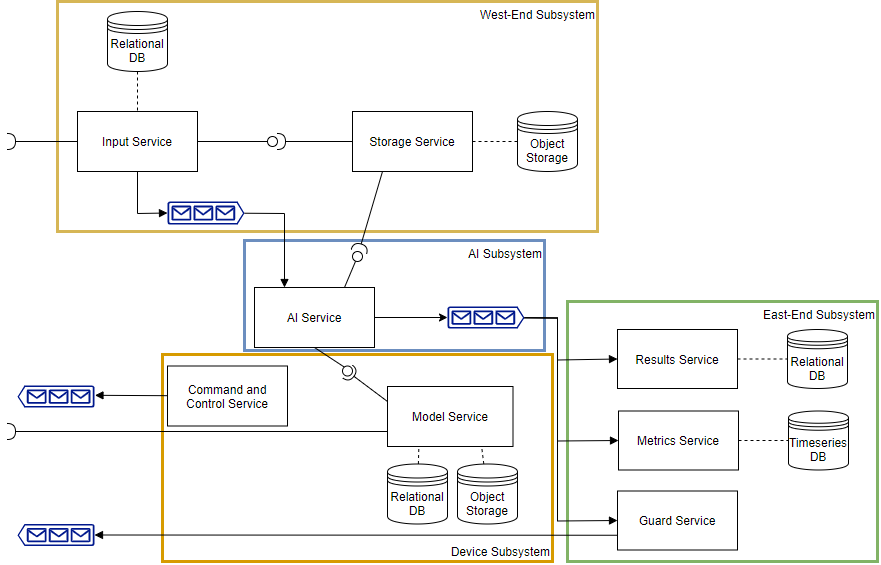
\includegraphics[width=150mm, keepaspectratio]{figures/architecture-redesigned.png}
\caption{A Birdnetes rendszer architektúrája}
\label{fig:birdnetes-components}
\end{figure}

%----------------------------------------------------------------------------
\subsubsection{IoT eszközök}
%----------------------------------------------------------------------------
Szőlőültetvényekben telepített eszközök, melyek adott időközönként publikálják állapotaikat egyéb metaadatokkal egy üzenetsoron.
Emellett folyamatosan hangfelvételt készítenek a beépített mikrofonjaikkal, mely hangfelvételekről egy másik belső szenzor eldönti,
hogy érdemes-e felküldeni a rendszerbe, ha igen, akkor egy másik üzenetsoron publikálják ezeket a hangfelvételeket.
Tartalmaznak még egy hangszórót is, mely a madarak elijesztését szolgálja.

%----------------------------------------------------------------------------
\subsubsection{Input Service}
%----------------------------------------------------------------------------
A kihelyezett IoT eszközök által felvett hangfájlok ezen a komponensen keresztül érkeznek be a rendszerbe.
Itt történik a hanganyaghoz tartozó metaadatok lementése az Input Service saját adatbázisába. 
Ilyenek például a beküldő eszköz azonosítója, a beérkezés dátuma vagy a hangüzenet rendszerszintű egyedi azonosítója.
Amint a szolgáltatás a berékezett üzenettel kapcsolatban elvégezte az összes feladatát, 
publikál egy üzenetet az MQTT üzenetsorra a többi kliensnek feldolgozásra.

%----------------------------------------------------------------------------
\subsubsection{AI Service}
%----------------------------------------------------------------------------
Az AI Service példányai fogadják az Input Service-től érkező üzeneteket és elkezdik klasszifikálni az abban található hanganyagot.
Meghatározzák, hogy a hanganyag mekkora valószínűséggel volt seregély hang vagy sem.
Ennek eredményét a hangminta egyedi azonosítójával együtt publikálják egy másik üzenetsoron.

%----------------------------------------------------------------------------
\subsubsection{Guard Service}
%----------------------------------------------------------------------------
A Guard Service feliratkozik az AI Service által publikált üzenetek témájára 
és valamilyen valószínűségi kritérium alapján eldönti, hogy a hangminta tartalmaz-e seregély hangot.
Ha igen, akkor az üzenetsoron küld egy riasztás parancsot a hanganyagot küldő eszköznek.

%----------------------------------------------------------------------------
\subsubsection{Command and Control Service}
%----------------------------------------------------------------------------
A Command and Control Service az előzőekkel ellentétben egyáltalán nem vesz részt a minták fogadásában, feldolgozásában vagy kezelésében.
Felelősége az eszközök és azok szenzorai állapotának menedzselése és követése.
Ezen keresztül lehet az egyes eszközöket ki- és bekapcsolni.
%----------------------------------------------------------------------------
\chapter{Tervek és alternatívák}
\label{chapt:birdmap-introduction}
%----------------------------------------------------------------------------
Ebben a fejezetben bemutatom a fejlesztés előtti állapotot, amikor a munkám elején a fontosabb vizualizációs alternatívákat értékeltem.

%----------------------------------------------------------------------------
\section{Tervezés}
%----------------------------------------------------------------------------
A munkám elején egyeztettem a seregély riasztó keretrendszert fejlesztő kollégákkal, 
hogy ki tudjam választani a vizualizáció szempontjából legfontosabb komponenseket.
A jellemző adatvizualizációs megoldások közül az alábbi hármat találtam kulcsfontosságúnak a következő célokra:
\begin{itemize}
    \item \textbf{Hőtérkép}. Hasznos lenne egy olyan felület, ahol az eszközök GPS koordinátái és a seregély detektálást jelző üzenetek alapján, meg lehetne jeleníteni a seregélyek hozzávetőleges előfordulásának helyeit és gyakoriságát egy térképen, hőtérképes formában.
    \item \textbf{Eszközállapotok}. Jelenleg a Command and Control mikroszolgáltatás felé indított kéréseken kívül, nincs lehetőség a kihelyezett eszközök állapotának vizsgálatára. Szükség lenne egy olyan felületre, ahol ezek állapotai láthatóak, esetleg dinamikusan is frissülnek.
    \item \textbf{Diagramok}. A hőtérképen kívül egyéb olyan diagramok is hasznosak lehetnek, ahol látható például, hogy melyik eszköz melyik percben észlelt madárhangot vagy, hogy egy eszköz összesen hány madárhangot észlelt. Minél több információ, annál jobb.
\end{itemize}
Ezeken kívül fontos követelmény volt még, hogy az alkalmazásom futtatható legyen Linux környezetben is, hogy az telepíthető legyen a Birbnetes Kubernetes \cite{kubernetes} klaszterébe.

Az alkalmazásom kapott egy nevet is, mely a Birbnetes-t és az említett hőtérképes ötletet ötvözve Birdmap lett.
\footnotetext{Microsoft Teams: Csevegő és gyülekezés tartó alkalmazás.}
%----------------------------------------------------------------------------
\section{Alternatívák}
%----------------------------------------------------------------------------
Az imént vázolt igények kielégítésére sok, széles körben alkalmazott megoldás létezik már, melyek jó példát mutattak a saját alkalmazásom fejlesztése során.

%----------------------------------------------------------------------------
\subsection{Grafana}
%----------------------------------------------------------------------------
A Grafana \cite{grafana} az egy nyílt forráskódú platformfüggetlen vizualizációs web alkalmazás.
Egy támogatott adatbázishoz csatlakoztatva különféle interaktív gráfokat és diagramokat generál.
A testreszabhatóság maximalizásának érdekében különböző, akár harmadik fél által készített, bővítmények használatát is támogatja, 
melyekkel új adatforrások és panel típusok integrálhatók. 
A \ref{fig:grafana}-es ábra egy jó példa arra, hogy hogyan néz ki egy általános Grafana felület.

\begin{figure}[!ht]
    \centering
    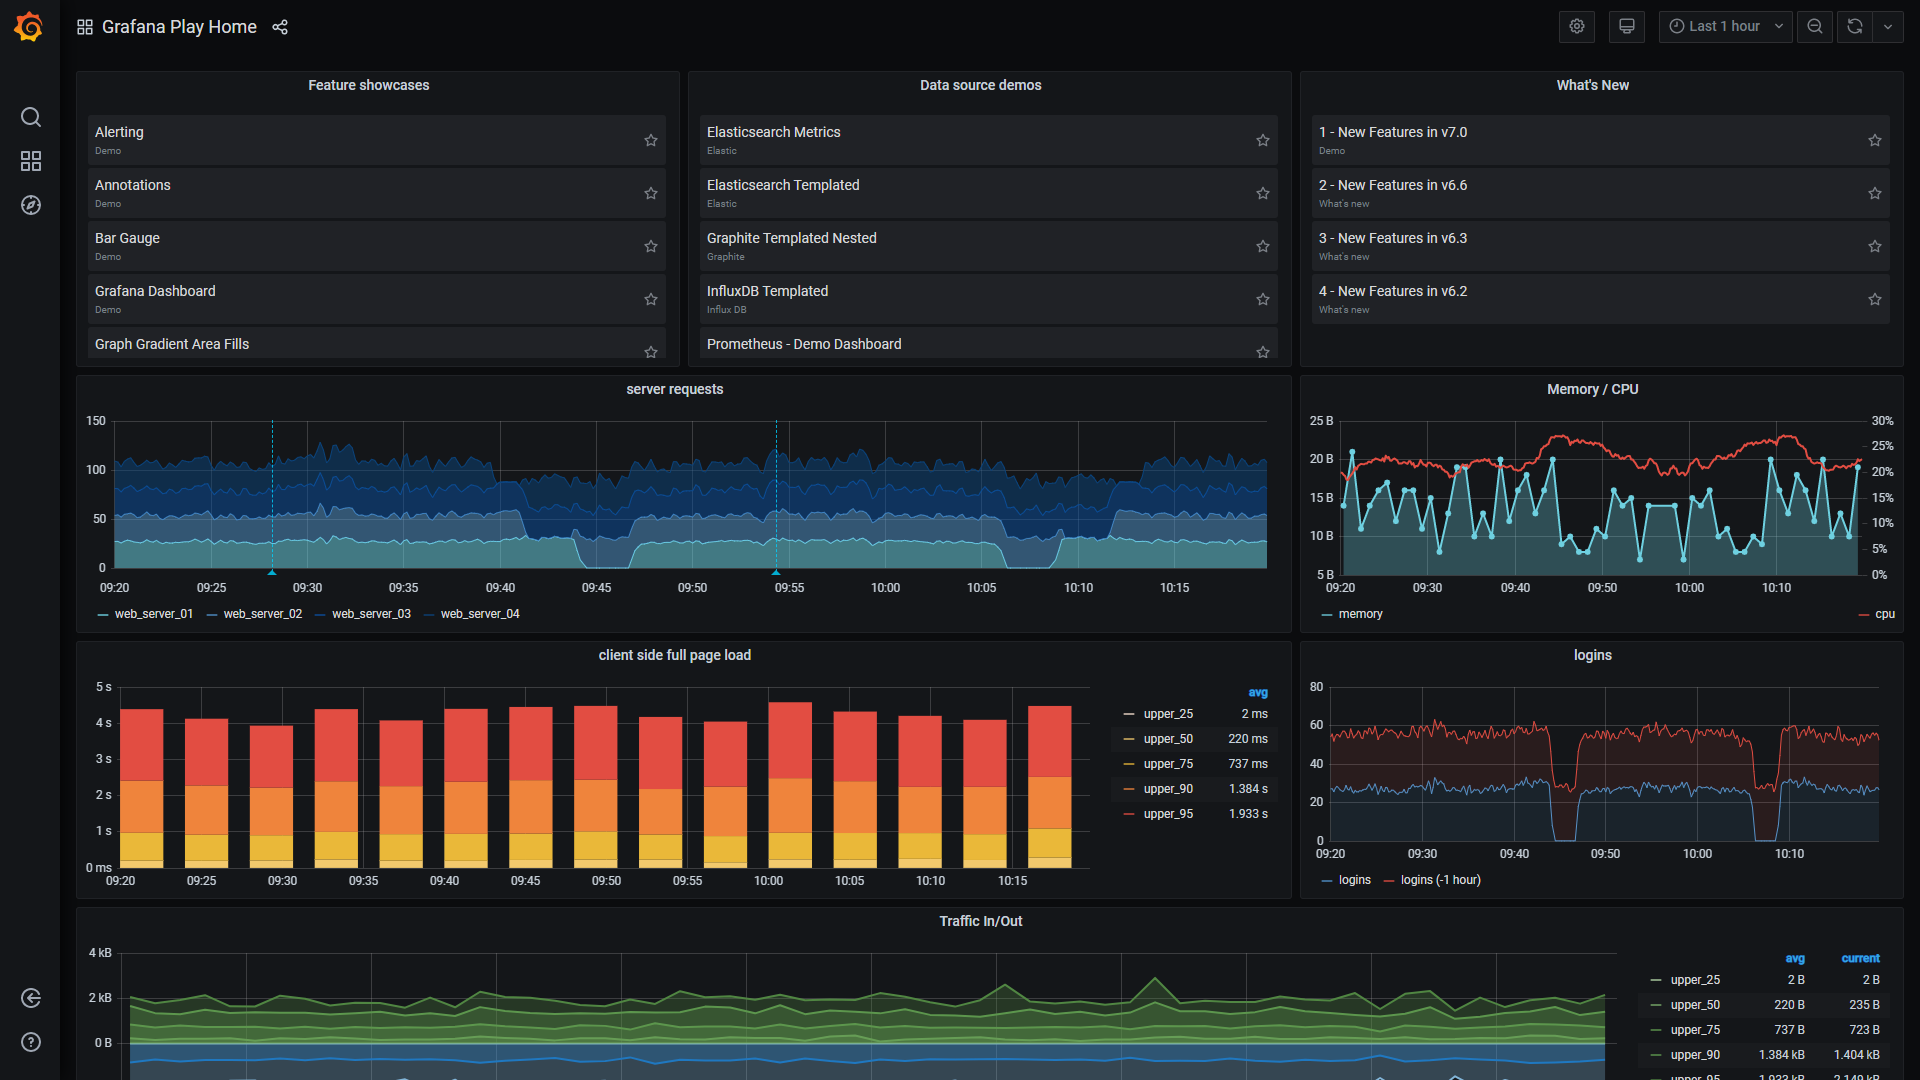
\includegraphics[width=150mm, keepaspectratio]{figures/grafana.png}
    \caption{A Grafana demo oldalának, a \url{https://play.grafana.org}-nak a felülete}
    \label{fig:grafana}
\end{figure}
    
%----------------------------------------------------------------------------
\subsection{Kibana}
%----------------------------------------------------------------------------
A Kibana \cite{kibana} jelentősen hasonlít a Grafanához, azonban amíg a utóbbit inkább az időben változó metrikák vizualizálására használják például processzor leterheltség vagy memória használat,
addig az előbbit elsődlegesen az Elasticsearch\footnote{Ingyenes és nyílt forráskódú index alapú keresőmotor} adatok, főként napló bejegyzések, analizálására használják.

\begin{figure}[!ht]
    \centering
    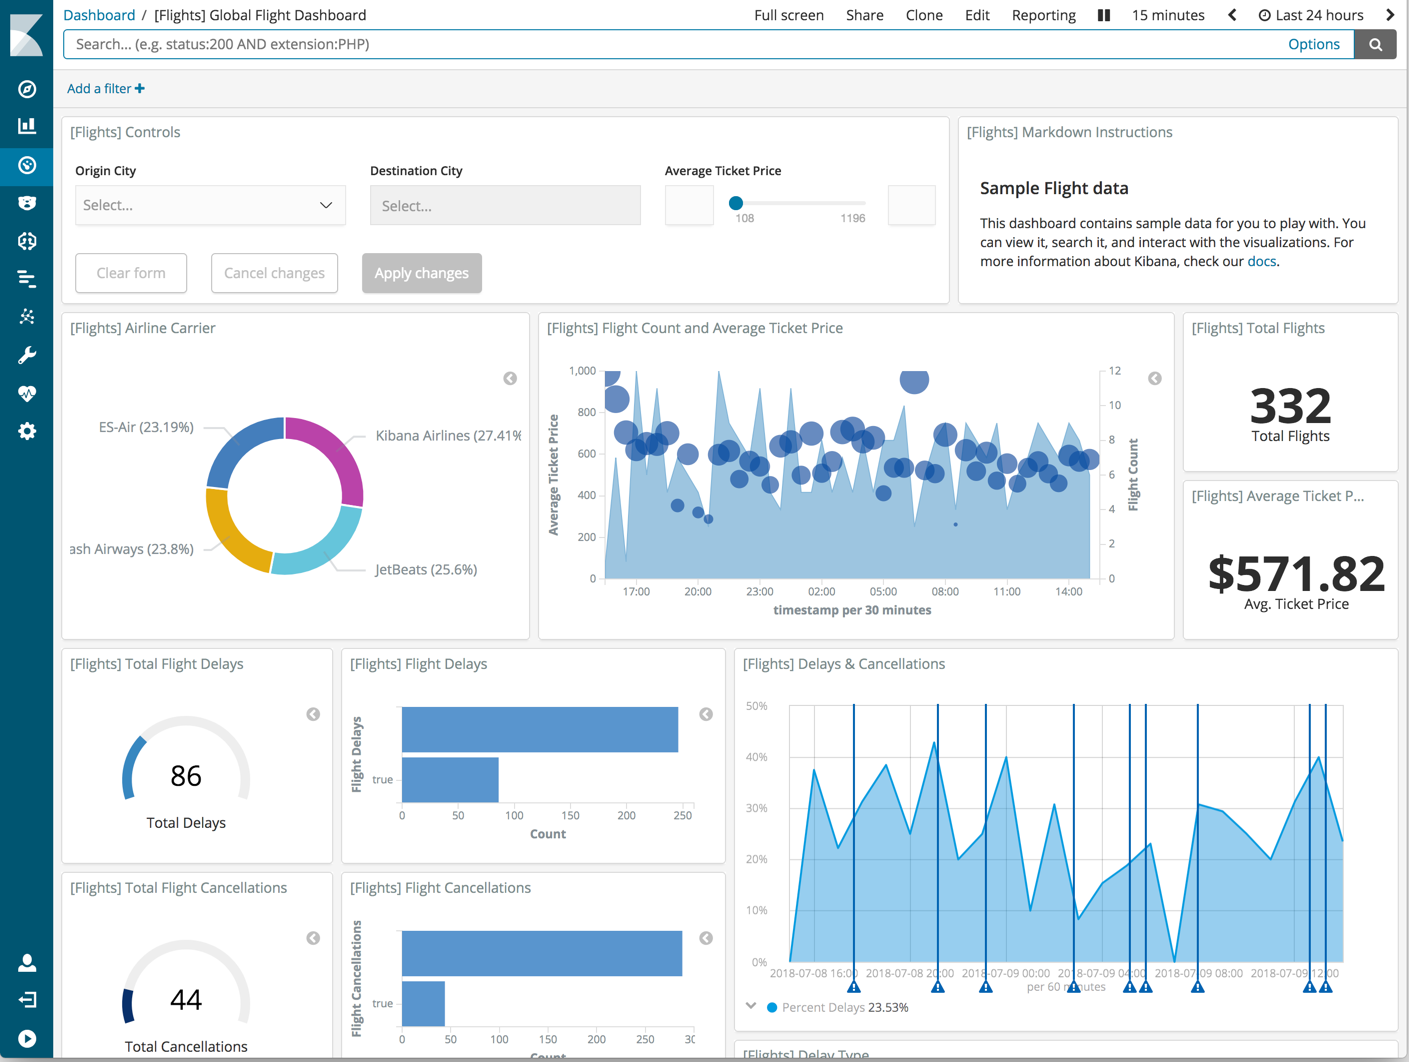
\includegraphics[width=150mm, keepaspectratio]{figures/kibana-dashboard.png}
    \caption{Egy példa a Kibana kezelőfelületére}
    \label{fig:kibana}
\end{figure}

%----------------------------------------------------------------------------
\subsection{Kubernetes Dashboard (Web UI)}
%----------------------------------------------------------------------------
A Kubernetes Dashboard \cite{kubernetes-dashboard} elsősorban nem a különböző adatok vizualizálását szolgálja, inkább a klaszter menedzselését próbálja egyszerűbbé és jobban áttekinthetővé tenni.
Azonban egy jó példa arra, hogy egy rendszer webes kezelőfelületének, milyennek is kell lennie.

\begin{figure}[!ht]
    \centering
    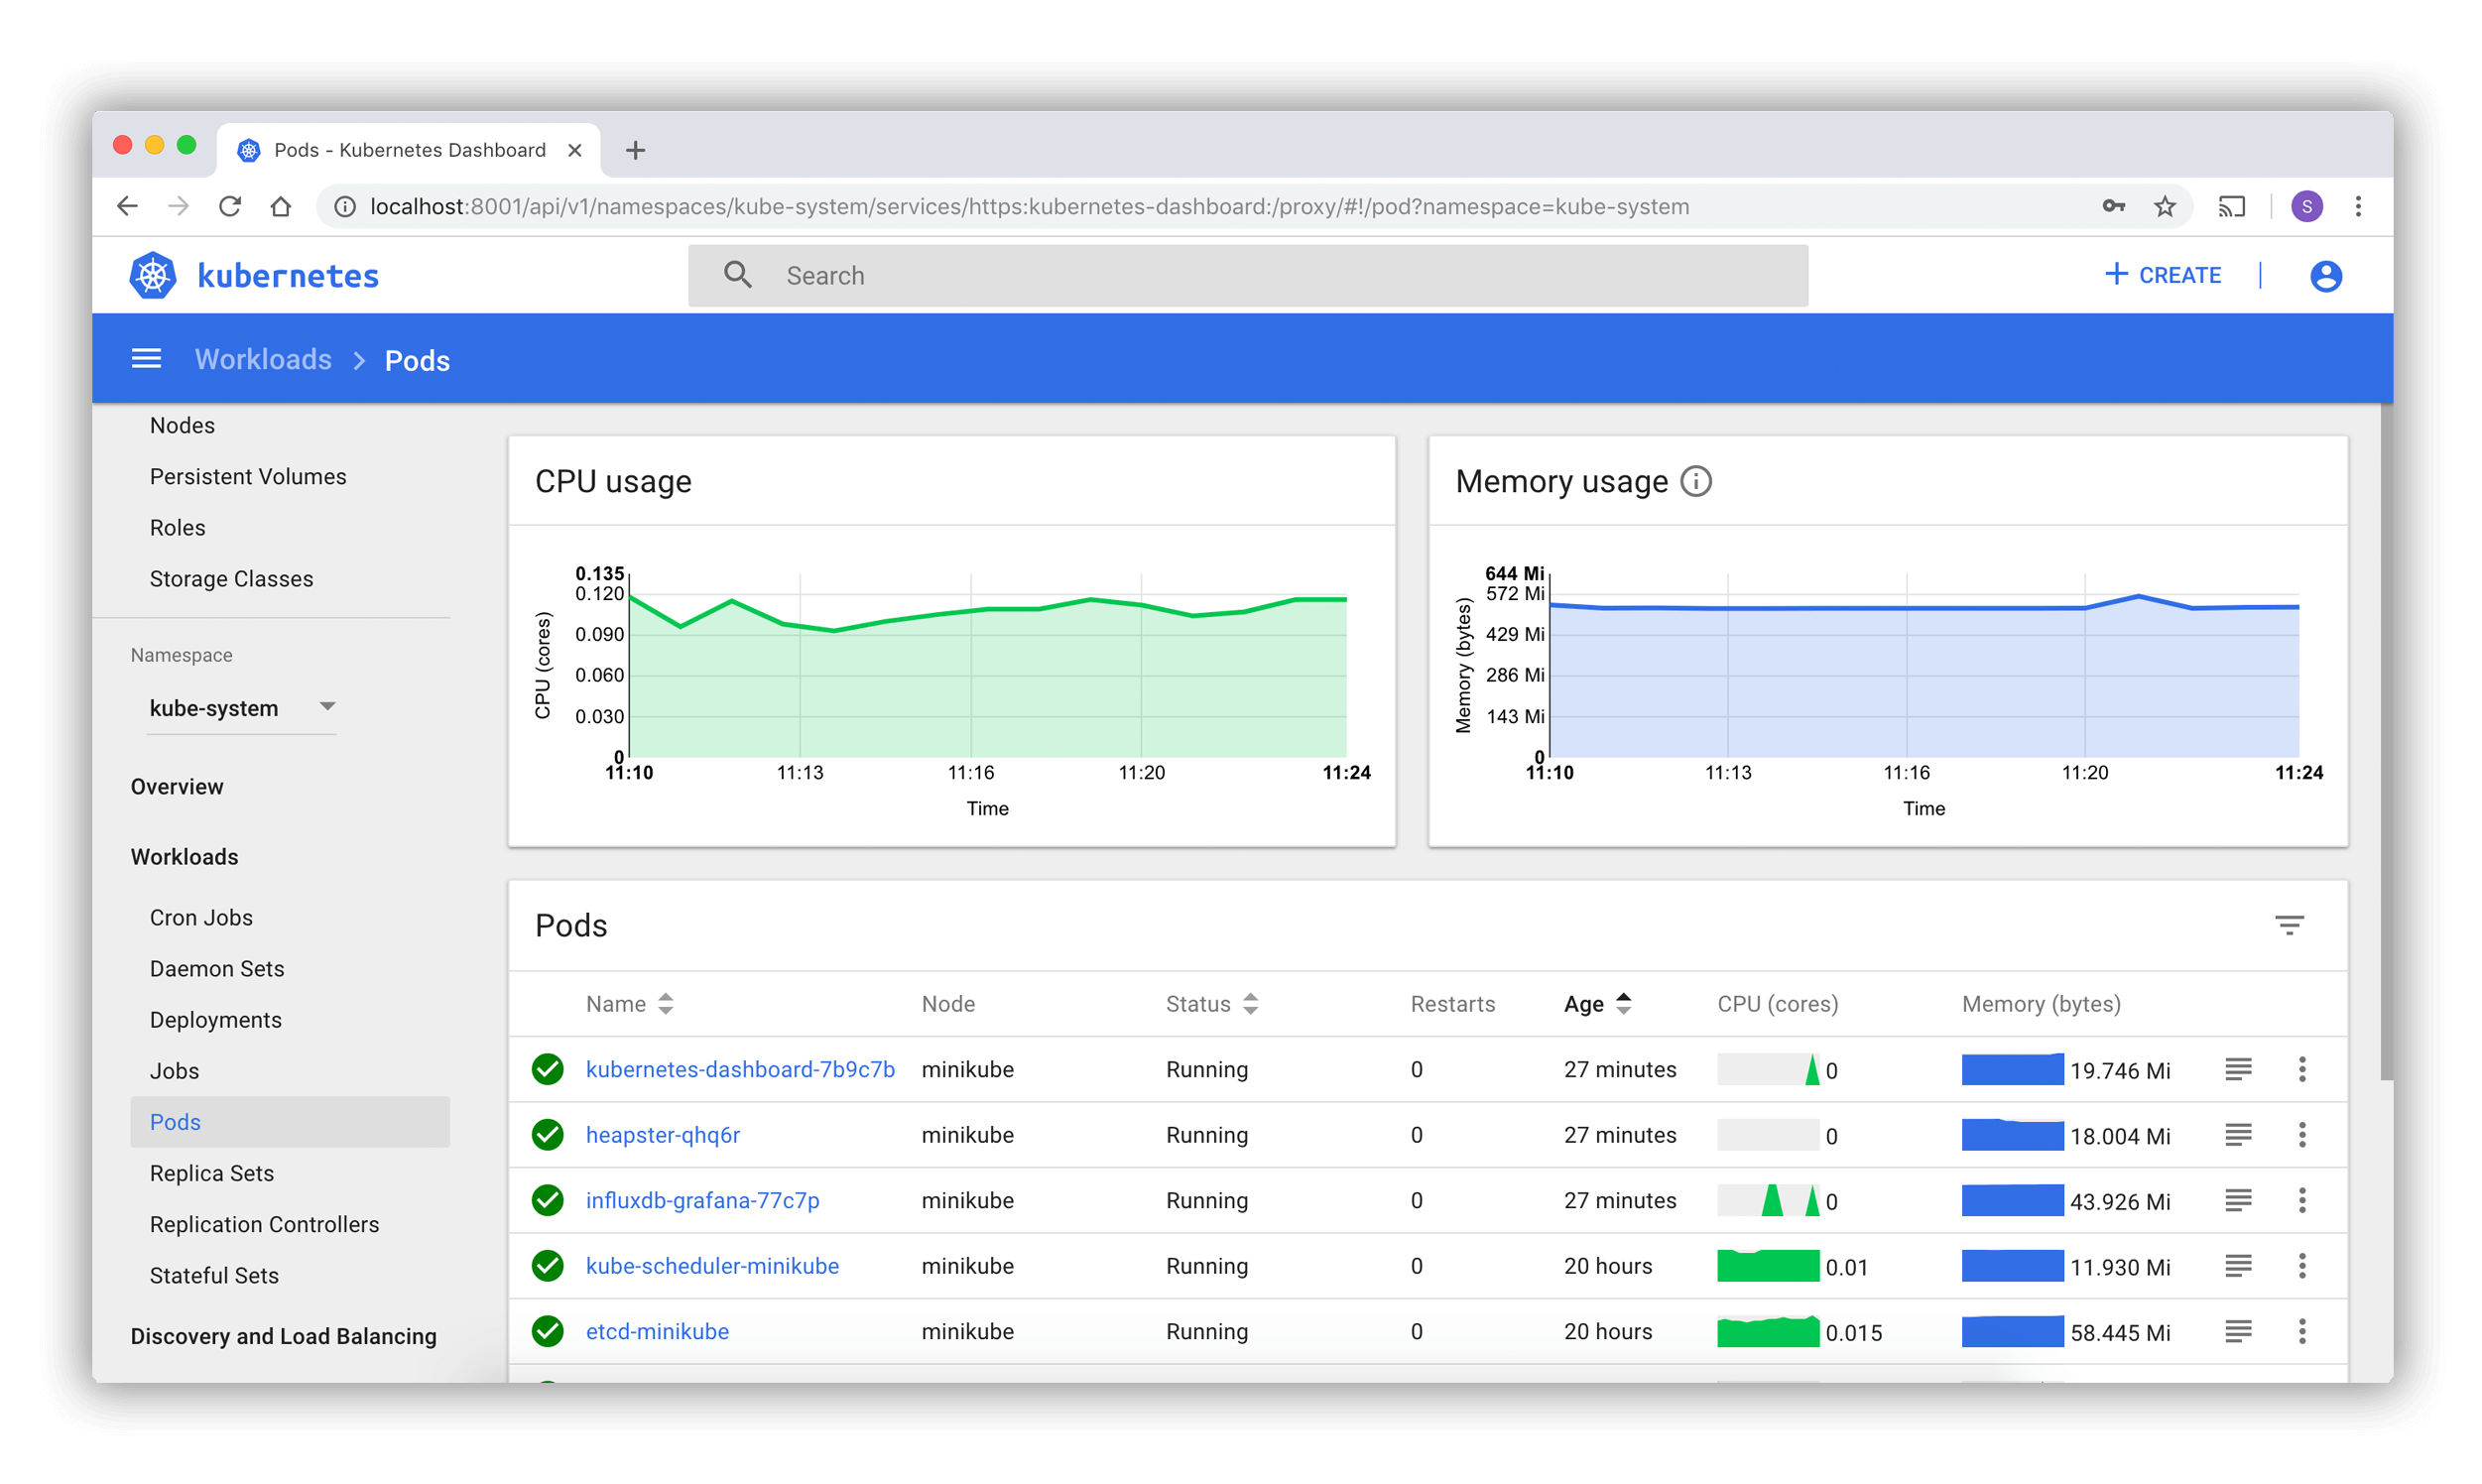
\includegraphics[width=150mm, keepaspectratio]{figures/kubernetes-dashboard.png}
    \caption{A Kubernetes Dashboard felülete}
    \label{fig:kibana}
\end{figure}
%----------------------------------------------------------------------------
\chapter{Használt technológiák}
\label{chapt:birdmap-technologies}
%----------------------------------------------------------------------------
Ezzel a fejezettel az a célom, hogy ismertessem a fejlesztés során, illetve az alkalmazásom által használt technológiákat,
hogy a következő fejezetekben alapozni tudjak ezeknek az ismeretére.

%----------------------------------------------------------------------------
\section{A fejlesztési folyamat technológiái}
%----------------------------------------------------------------------------
Ebben a szakaszban azokat az eszközöket, alkalmazásokat mutatom be, melyeket a fejlesztés során használtam. 

%----------------------------------------------------------------------------
\subsection{Git}
%----------------------------------------------------------------------------
A Git\cite{git} egy verziókezelő rendszer. Használatával a felhasználó le tudja menteni egy adott fájlrendszerben található fájlok állapotát.
Megkönnyíti az egy projekten dolgozó programozók közötti kooperációt. Manapság lassan elképzelhetetlen a fejlesztés valamilyen verziókezelő használata nélkül.

%----------------------------------------------------------------------------
\subsection{Trello}
%----------------------------------------------------------------------------
A Trello\cite{trello} egy webes lista készítő és kezelő alkalmazás. 
Azért használtam a fejlesztés során, mert szerettem volna egy helyet, ami tükrözi a fejlesztés állapotát, ahova le tudom írni az alkalmazással kapcsolatos ötleteimet.
Különböző listákban tároltam a fejlesztésre váró és a kész feladatokat szerver, kliens és egyéb szerint.

\begin{figure}[!ht]
    \centering
    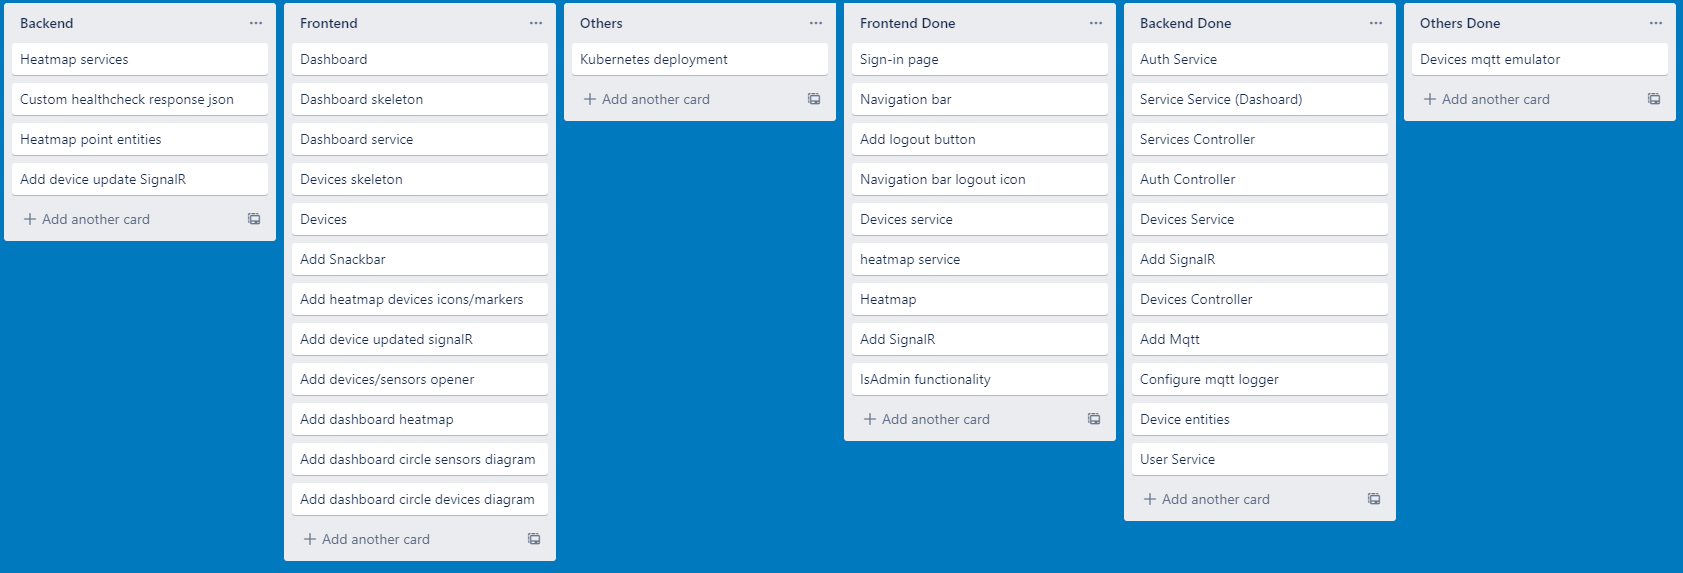
\includegraphics[width=150mm, keepaspectratio]{figures/trello-cropped.png}
    \caption{Egy példa állapot a Trello felületére a fejlesztés során}
    \label{fig:trello}
\end{figure}

%----------------------------------------------------------------------------
\subsection{Visual Studio}
%----------------------------------------------------------------------------
A Visual Studio\cite{vs} a Microsoft fejlesztőkörnyezete. Jól alkalmazható a .NET keretrendszer technológiáival, ezért ezt használtam a szerveroldal fejlesztése során.

%----------------------------------------------------------------------------
\subsection{Visual Studio Code}
%----------------------------------------------------------------------------
Egy másik Microsoft termék, viszont a fentivel ellentétben a Visual Studio Code\cite{vs-code} inkább szövegszerkeztő, mint fejlesztőkörnyezet.
Ennek köszönhetően jelentősen gyorsabb és egyszerűbb a használata. Különféle bővítmények használatával nagyon jó program nyelv támogatottságot lehet elérni.
Többek között ezen okok miatt preferáltam a kliensoldal fejlesztésére. 

%----------------------------------------------------------------------------
\section{Backend technológiák}
%----------------------------------------------------------------------------
Ebben a szakaszban a szerveroldal megvalósítására használt .NET technológiákat mutatom be. A választásom több ok miatt esett a .NET keretrendszer használatára.

Egyrészt úgy gondoltam, hogy az alkalmazásom fajsúlyosabb részét inkább a kliensoldal fogja képezni ezért, hogy arra több energiát tudjak fordítani, valami olyat választottam,
amivel már foglalkoztam korábban, amivel gyorsabban és rutinosabban megy a fejlesztés.

Másrészt nemrég jelent meg a .NET új 5-ös verziója, melynek használatával jelentős teljesítmény javulást ígértek több területen is, és úgy gondoltam, hogy ez a projekt tökéletes lenne
ennek próbatételére.

Mindemellett a .NET teljesen platformüggetlen, mely az egyik legfontosabb követelmény volt az alkalmazással szemben.

%----------------------------------------------------------------------------
\subsection{ASP.NET Core}
%----------------------------------------------------------------------------
Az ASP.NET Core a .NET család ingyenes, nyílt forráskódú webes keretrendszere. Gyors és moduláris fejlesztést tesz lehetővé, mely főként a NuGet csomagoknak köszönhető.
Használatána egyik előnye, hogy ugyan az a C\# kód tud futni a szerver éa a kliens oldalon, de támogat más kliens oldali keretrendszereket is, mint például az Angular-t, a Vue.js-t
vagy a React.js-t.

%----------------------------------------------------------------------------
\subsection{Entity Framework Core}
%----------------------------------------------------------------------------
Az Entity Framework Core (röviden EF Core) egy objektum-relációs leképező keretrendszer a .NET-hez. Az adatbázissal való kommunikációt könnyítését szolgálja. 
Használatával C\#-ban lehet adatbázis lekérdezéseket írni a LINQ (Language-Integrated Query) segítségével.

%----------------------------------------------------------------------------
\subsection{SignalR}
%----------------------------------------------------------------------------
A SignalR egy .NET szoftvercsomag, mely lehetővé teszi a szerveroldal számára a kliensekkel való aszinkron kommunikációt.
A szerver valós időben tud értesítéseket küldeni a kliensek számára, amelyek feliratkoztak az ilyen eseményekre.

%----------------------------------------------------------------------------
\subsection{MQTT.NET}
%----------------------------------------------------------------------------
Az MQTT.NET is egy .NET szoftvercsomag, mely a Birdnetes által is használt, a \ref{subsect:mqtt}-es alfejezetben bemutatott MQTT kommunikáció C\# nyelvű megvalósítását szolgálja.

%----------------------------------------------------------------------------
\section{Frontend technológiák}
%----------------------------------------------------------------------------
Ebben a szakaszban a kliensoldalhoz használt technológiákat mutatom be. 
Választásomnál fő motiváció az volt, hogy szerettem volna valami újat kipróbálni, aminek nincs köze a .NET technológiákhoz.

%----------------------------------------------------------------------------
\subsection{React.js}
%----------------------------------------------------------------------------
A React.js\cite{react} egy JavaScript szoftvercsomag, melyet webes felületek fejlesztésére használnak.
Fő építő elemei a komponensek, melyek elszeparált újrafelhasználható felület egységek.
Használatának egyik előnye, hogy automatizált az állapot kezelés, tehát ha változik egy komponens állapota, akkor a React újra-rendereli azt.

%----------------------------------------------------------------------------
\subsection{Material UI}
%----------------------------------------------------------------------------
A Material\cite{material} elsősorban egy kezelőfelület tervezési útmutató a Google által, melyet követve szép és minőségi felületeket lehet készíteni.

A Material UI\cite{material-ui} egy szoftvercsomag, mely ezeket az útmutatásokat követő egyszerű React komponenseket tartalmaz.
Alkalmazásával könnyő esztétikus felhasználói felületeket készíteni, minimalizált a CSS használattal. 

%----------------------------------------------------------------------------
\subsection{Apexcharts}
%----------------------------------------------------------------------------


%----------------------------------------------------------------------------
\subsection{Google Maps Api}
%----------------------------------------------------------------------------
%----------------------------------------------------------------------------
\chapter{Szerver oldal}
\label{chapt:birdmap-backend}
%----------------------------------------------------------------------------
Ebben a fejezetben bemutatom a szerveroldal architektúráját, felépítését. Ismertetem a különböző szoftver komponensek feladatát.

%----------------------------------------------------------------------------
\section{Architektúra}
%----------------------------------------------------------------------------
A szerveroldal fejlesztésénél a háromrétegú architektúrát alkalmaztam, melynek lényege, hogy az alkalmazást logikailag három elkülönülő részre bontjuk:
\begin{itemize}
    \item \textbf{Adat elérési réteg}. Ez a rész felel a tárolt entitások modell definícióiért, illetve azoknak a kiolvasásáért, tárolásáért egy adatbázisból vagy fájlrendszerből.
    \item \textbf{Megjelenítési réteg}. Ezen réteg feladata a kliensoldal közvetlek kiszolgálása. Bármilyen irányú kommunikáció a kliensek felé ezen a rétegen keresztül történik.
    \item \textbf{Üzleti logikai réteg}. Minden ami nem a közvetlen kommunikációért, megjelenítésért vagy adat elérésért, tárolásért felel, az ide kerül.
    A fenti két réteg között helyezkedik el és feladata a különböző folyamatok értékelése és futtatása, valamint az adatok feldolgozása.
\end{itemize}

Az ASP.NET Core beépítetten támogatja a dependency injection-t, mely a \verb+Startup+ osztály \verb+ConfigureServices+ metódusával konfigurálható.
Én minden rétegbe tettem egy ilyen \verb+Startup+ osztályt, hogy azok feleljenek a saját szolgáltatásaik konfigurálásáért és regisztrálásáért.

%----------------------------------------------------------------------------
\section{Adat elérési réteg}
%----------------------------------------------------------------------------
Az adatelérést az Entity Framework Core segítségével oldottam meg. Telepítettem egy MSSQL adatbázis szervert a számítógépemre, melynek csatlakozási paramétereivel
a \verb+Startup+ osztályban felkonfigurálom az EF Core által nyújtott \verb+DbContext+ saját leszármazott változatát. 
Így csak az entitások elkészítése és azok alapértelmezett értékeinek az adatbázisba való feltöltése marad hátra.

%----------------------------------------------------------------------------
\subsection{Entitások}
%----------------------------------------------------------------------------
Mivel az adatok nagy részét külső szolgáltatások fogják nyújtani, így lokálisan összesen két entitás létrehozására volt szükség. 
Az egyik a \verb+User+, mely az alkalmazás felhasználóinak adatait tárolja. 
A másik a \verb+Service+, mely a külső szolgáltatások adatainak tárolását szolgálja, amelyeket azért tárolok az adatbázisban és nem mondjuk a konfigurációs fájlban,
mert szerettem volna, hogyha a kezelőfelületen lehetne őket szerkeszteni, törölni.

\lstset{style=sharpc, morekeywords={record, get, set}}
\begin{lstlisting}[caption=A User és a Service modell]
    public record User
    {
        public int Id { get; set; }
        public string Name { get; set; }
        public byte[] PasswordHash { get; set; }
        public byte[] PasswordSalt { get; set; }

        public Roles Role { get; set; }

        public bool IsFromConfig { get; set; }
    }

    public record Service
    {
        public int Id { get; set; }
        public string Name { get; set; }
        public Uri Uri { get; set; }

        public bool IsFromConfig { get; set; }
    }
\end{lstlisting}

Az alkalmazás használata szempontjából a felhasználók két csoportba oszlanak.
Vannak adminisztrátor és sima felhasználók, utóbbi csak az adatok olvasására, míg előbb azok módosítására is jogosult.
A \verb+Role+ mező ennek a megkülönböztetsnek a jelzője.

%----------------------------------------------------------------------------
\subsection{Seedelés}
\label{subsect:seeding}
%----------------------------------------------------------------------------
Az alkalmazás konfigurációs fájljából meg lehet adni alapértelmezett felhasználókat és szolgáltatásokat.
Ezeknek megkülönböztetésére szolgál az entitások \verb+IsFromConfig+ mezője.
A szerver indítása legelején, megvizsgálja, hogy létezik-e az adatbázis és ha igen kitöröl minden olyan entitást ahol az \verb+IsFromConfig+ mező igaz.
Majd hozzáadja az újonnan beolvasott értékeket.

%----------------------------------------------------------------------------
\section{Üzleti logikai réteg}
%----------------------------------------------------------------------------
Ebben a rétegben található meg a szerver legtöbb szolgáltatása. It vannak implementálva a Birdnetes Command and Control és Input komponensekkel kommunikáló szolgáltatások is, 
melyeket azok OpenAPI leírói alapján az NSwag\cite{nswag} alkalmazással generáltam. Az OpenAPI a klienseken kívül definiálja még az azok által használt modelleket is.
A Command and Control által használt \verb+Device+ modell tartalmazza annak egyedi azonosítóját, státuszát, koordinátáit és a használt szenzorok listáját, 
melyeknek szintén van egy modellje \verb+Sensor+ néven. Ennek szintén van azonosítója és státusza. Az Input szolgáltatásnak is van saját modellje, 
amely a hangüzenetek metaadatait reprezentálja. Többek között tartalmazza a kihelyezett eszköz egyedi azonosítóját és a hangüzenet keltének dátumát. 

Ugyan itt található meg a \verb+User+ és \verb+Service+ entitások létrehozásáért, olvasásáért, szerkesztéséért és törléséért felelős szolgáltatások is.
Valamint itt található még az autentikációért felelős szolgáltatás is. A felhasználók jelszavainak tárolására a HMAC (Hash-based Message Authentication Code) algorithmust, 
pontosabban annak a \verb+HMACSHA512+\cite{hmacsha512} C\# implementációját használtam.

Minden jelszóhoz generálok egy egyedi kulcsot és azzal egy hash-t, majd ezeket tárolom a \verb+User+ modell \verb+PasswordSalt+ és \verb+PasswordHash+ mezőiben.
Amikor egy felhasználó be akar jelentkezni először megvizsgálom, hogy egyáltalán létezik-e az adatbázisban az adott nevű felhasználó, 
ha igen, akkor a megadott jelszóból az imént említett folyamattal generált kulcsot és hash-t összehasonlítom az adatbázisban tárolttal.

%----------------------------------------------------------------------------
\subsection{Kommunikációs Szolgáltatások}
%----------------------------------------------------------------------------
A kliensoldal frissítésére több megoldás is létezik. Például bizonyos időközönként lehetne kéréseket indítani a szerver felé a friss adatok megszerzéséért.
Egy másik megoldás a SignalR használata, amellyel a klienseket eseményvezérelten lehet értesíteni, megvalósítja a kétoldalú kommunikációt.
Így a kliensek csak akkor indítanak kéréseket amikor az adat tényleg változott. Ezzel a technológiával oldottam meg például, hogy az eszközök állapotainak változására
frissüljön a felület.

Egy másik szerveroldalon használt szolgáltatás a Birdnetes MQTT kommunikációért felelős szolgáltatás, 
mely felregisztrál a \ref{subsect:birdnetes-ai-service}-as alfejezetben bemutatott AI Service által publikált üzenetekre.
Ezekben az üzenetekben található a hanganyagok egyedi azonosítója, illetve azok seregélytől való származásának valószínüsége.
Ha a szolgáltatás kap egy ilyen üzenetet akkor lekérdezi a \ref{subsect:birdnetes-input-service}-es alfejezetben bemutatott Input Service-től
a hanganyag azonosítójához tartozó metaadatokat. 
Ezekből felhasználva a kihelyezett eszköz azonosítóját, a hanganyag beérkezésének dátumát és az említett valószínüséget új üzenetek készülnek, melyeket egy pufferben tárolódnak.
Ezt a folyamatot a \ref{fig:birdmap-mqtt-service}-es ábra szemlélteti.

\begin{figure}[!ht]
    \centering
    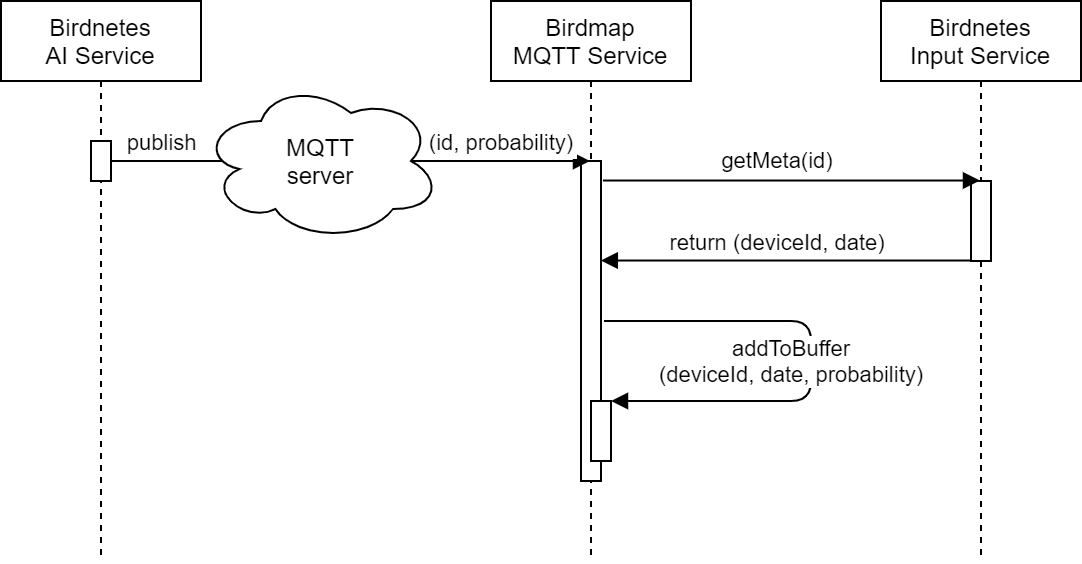
\includegraphics[width=150mm, keepaspectratio]{figures/mqtt-communication-sequence.png}
    \caption{A Birdmap MQTT szolgáltatásának szekvenciája}
    \label{fig:birdmap-mqtt-service}
\end{figure}

A puffer tartalmát másodperces gyakorisággal elküldöm a klienseknek a SignalR segítségével. 
Azért van szükség a puffer használatára, mert az MQTT-n érkezett üzenetek gyakorisága akár miliszekundum nagyságrendű is lehet. 
Míg a szerver képes is az üzeneteket feldolgozni, ha ezeket rögtön tovább küldeném a kliensek felé, azok nem biztos, hogy képesek lennének rá.

%----------------------------------------------------------------------------
\section{Megjelenítési réteg}
%----------------------------------------------------------------------------
A fejezet elején említett \verb+Startup+ osztály ebben a rétegben található, itt kerülnek az egyes szolgáltatások regisztrálásra.
Itt történik a \ref{subsect:seeding} fejezetben leírt adatbázis seedelése is.

Többek között a naplózás is itt kerül inicializálásra, mely az NLog saját konfigurációs fájljával történik.
Meg lehet adni különböző szűrőket és kimeneteket, amellyel szelektálni lehet, hogy az egyes naplózott események hova kerüljenek.
Például az MQTT szolgáltalás napló bejegyzéseit a \ref{lst:nlog-config} lista alapján szűrtem.
Minden \verb+Debug+ szintől nagyobb és \verb+Error+ szinttől kisebb bejegyzés, mely tartalmazza az \verb+Mqtt+ kulcsszót az \verb+mqttFile+ azonosítójú fájlba kerül.

\lstset{style=xml, morekeywords={targets, target, xsi:type, name, fileName, layout, rules, logger, name, minlevel, maxlevel, writeTo, final}}
\begin{lstlisting}[caption=Az NLog.config fájl egy részlete, label=lst:nlog-config]
<targets>
    ...
    <target xsi:type="File" name="mqttFile" fileName="${basedir}Logs/birdmap-mqtt-${shortdate}.log"
        layout="..." />
    ...
</targets>

<rules>
    ...
    <logger name="*.*Mqtt*.*" minlevel="Trace" maxlevel="Warning" writeTo="mqttFile" final="true"/>
    ...
</rules>
\end{lstlisting}

A \verb+Startup+ osztály másik metódusa a \verb+Configure+, mellyel a HTTP kérések csővezetéke konfigurálható.
Azaz, hogy egy kérés-t milyen sorrendben dolgozzák fel a regisztrált szolgáltatások.
A szerveroldali kivételkezelésre szánt szolgáltatás, az \verb+ExceptionHandlerMiddleware+ is itt van használva, 
amely elkap minden kivételt, amit a csővezeték további részei dobtak és JSON formátumban visszaadja azokat a kliensnek.

Továbbá az NSwag\cite{nswag} szoftvercsomag segítségével regisztrálok egy szolgáltatást, 
mely a szerveroldalon található kontrollereket felhasználva generál egy OpenAPI specifikációt és annak egy Swagger UI\cite{swagger-ui} felületet,
ahol a végpontok kipróbálhatóak, tesztelhetőek kliensoldal nélkül is.

\begin{figure}[!ht]
    \centering
    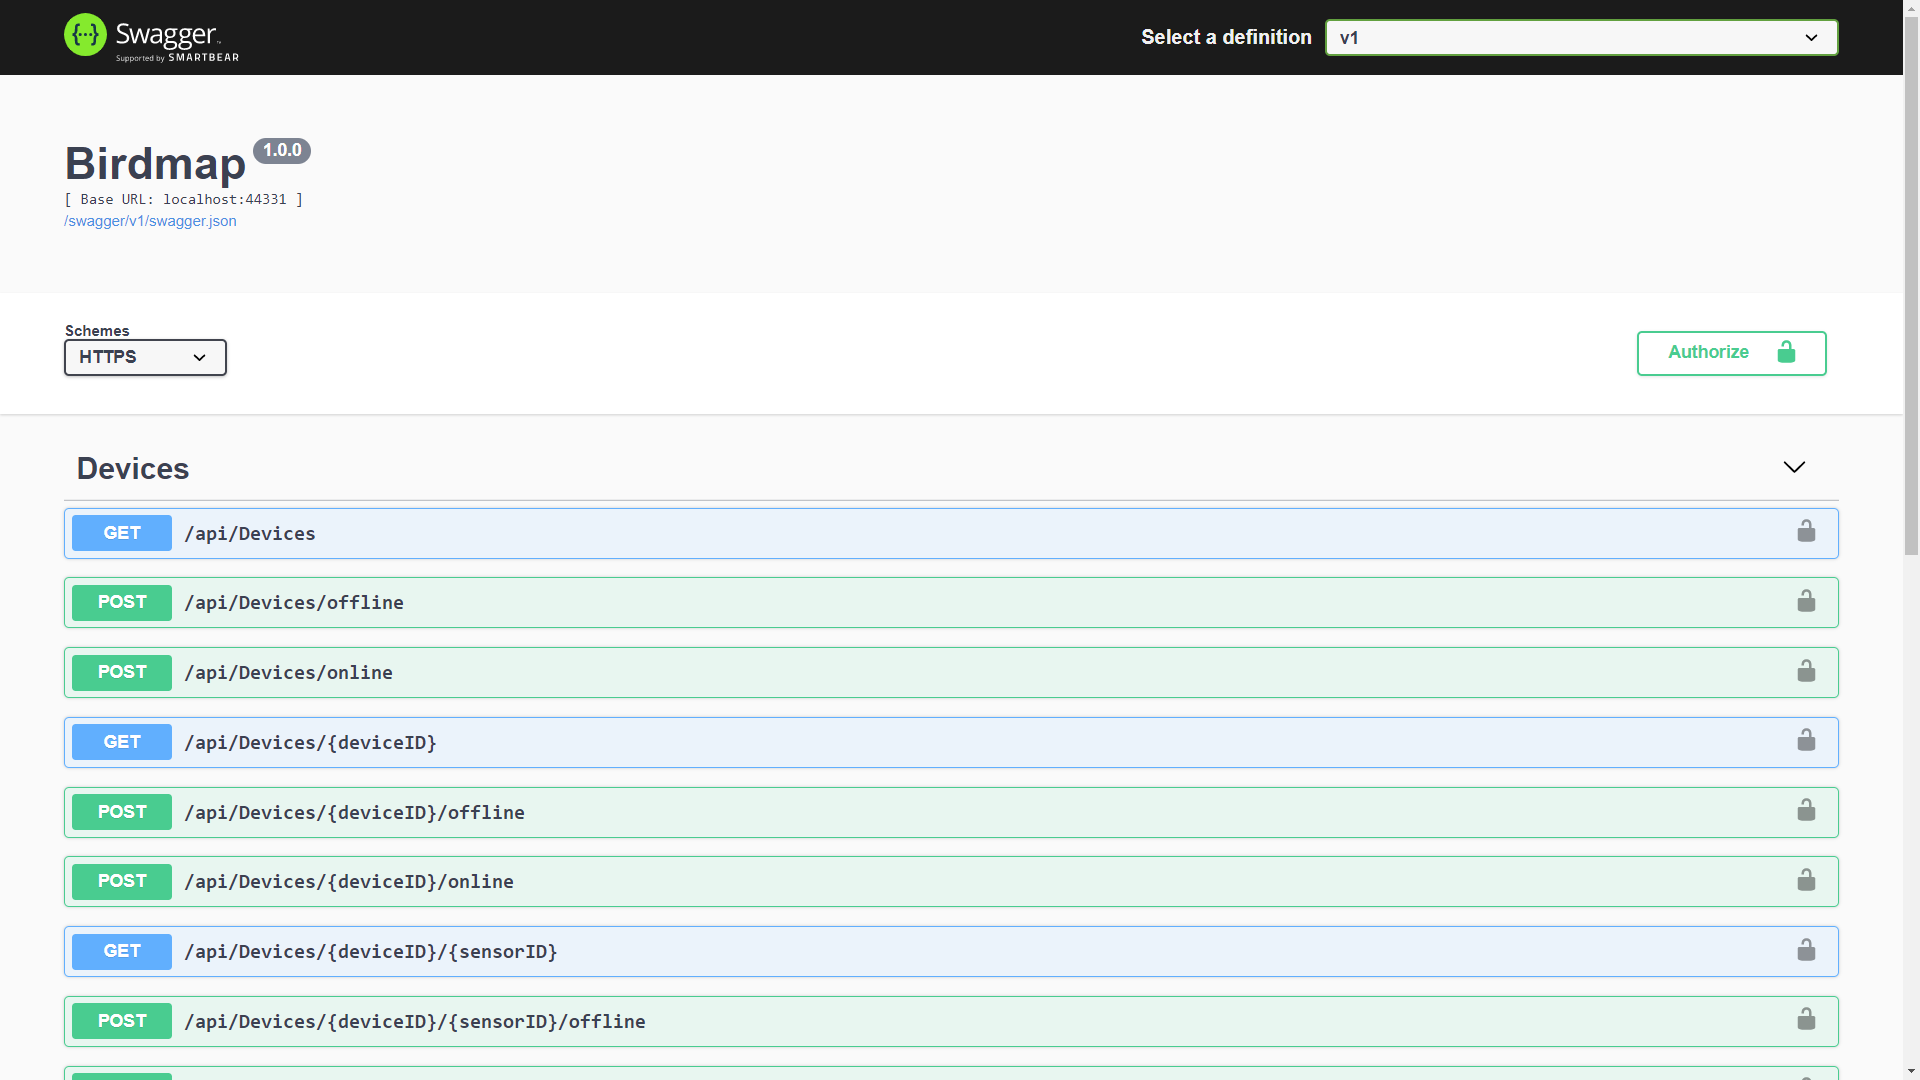
\includegraphics[width=150mm, keepaspectratio]{figures/swagger-ui.png}
    \caption{Az alkalmazásom Swagger felülete}
    \label{fig:swagger-ui}
\end{figure}

%----------------------------------------------------------------------------
\subsection{Kontrollerek}
%----------------------------------------------------------------------------
A kontrollerek határozzák meg, hogy a szerveroldalon milyen végpontokat, milyen paraméterekkel lehet meghívni, ahhoz milyen jogosultságok kellenek.
A jogosultságok kezelését a JSON Web Token-ekkel oldottam meg. A fejlasználó bejelentkezéskor kap egy ilyen token-t, 
amelyben tárolom a hozzá tartozó szerepet. A \ref{lst:devices-controller}-as listában látszik, hogy hogyan használom ezeket a szerepeket.
A \verb+DevicesController+ végpontjait alapértelmezetten \verb+User+ és \verb+Admin+ jogosultságú felhasználó hívhatja, az "api/devices/online" végpontot azonban csak \verb+Admin+ jogosultságú.
Hasonló képpen oldottam meg ezt a többi kontrollernél is. A \verb+User+ felhasználók csak olyan végpontokat hívhat, mely kizárolag az állapotok olvasásával jár.
Az \verb+Admin+ felhasználók hívhatnak bármilyen végpontot.

\lstset{style=sharpc, morekeywords={record, async}}
\begin{lstlisting}[caption=Az eszköz kontroller és annak "online" végpontja, label=lst:devices-controller]
    [Authorize(Roles = "User, Admin")]
    [ApiController]
    [Route("api/[controller]")]
    public class DevicesController : ControllerBase
    {
        [Authorize(Roles = "Admin")]
        [HttpPost, Route("online")]
        public async Task<IActionResult> Onlineall()
        {
            ...
        }
        ...
    }
\end{lstlisting}

Controllersw
Dtos
mapper
%----------------------------------------------------------------------------
\chapter{Kliens oldal}
\label{chapt:birdmap-frontend}
%----------------------------------------------------------------------------
Ebben a fejezetben bemutatom a kliensoldal architektúráját. Ismertetem a különböző komponensek felépítését.

%----------------------------------------------------------------------------
\section{Architektúra}
%----------------------------------------------------------------------------
Az alkalmazásnak minden oldala egy külön React komponens, mely mindegyikének saját mappája van a főkönyvtár alatt, 
ahol az egyes oldalak által használt szolgáltatások és egyéb komponensek találhatóak.
A közösen használt szolgáltatások és komponensek a common mappába kerültek.

A kliensoldal belépési pontja az \verb+App.js+ fájlban található \verb+App+ komponens.
Itt egy React \verb+Switch+-ben fel van sorolva az összes oldal komponense azok elérési útvonalai szerint.
Ezt szemlélteti a \ref{lst:react-switch}-es lista.
Az a komponens jelenik meg a felületen, amelyiknek \verb+path+ mező értéke megegyezik az URL-ben találhatóval.

\begin{lstlisting}[style=jsx, caption=Az App.js Switch tartalma., label=lst:react-switch]
<Switch>
    <PublicRoute exact path="/login" component={AuthComponent} />
    <AdminRoute exact path="/logs" component={LogsComponent} />
    <DevicesContextProvider>
        <PrivateRoute exact path="/" component={DashboardComponent} />
        <PrivateRoute exact path="/devices/:id?" component={DevicesComponent} />
        <PrivateRoute exact path="/heatmap" component={HeatmapComponent} />
    </DevicesContextProvider>
</Switch>
\end{lstlisting}

Hozzáférés szempontjából háromfajta oldalt különböztetünk meg:
\begin{itemize}
    \item \textbf{Publikus oldal}. Az oldal bejelentkezés nélkül is látogatható.
    \item \textbf{Privát oldal}. Az oldal csak bejelentkezés után látogatható.
    \item \textbf{Admin oldal}. Az oldalt csak bejelentkezett admin felhasználók látogathatják.
\end{itemize}

Ezek alapján készítettem két generikus komponenst. Az egyik a \verb+DefaultLayout+ komponens, mely az oldal alapértelmezett elrendezéséért felel.
Paraméterében át lehet adni egy másik megjeleníteni kívánt komponenst, melyet a fejléc alatt jelenít meg.
Mivel minden komponens ebbe az bázis komponensbe van csomagolva, így akárhova navigálunk az oldalon a felület mindig egységes marad.

A másik komponens a \verb+PredicateRoute+, melynek paraméterében meg lehet adni egy feltételt, illetve egy másik komponenst.
Ha a feltétel hamis akkor átirányítja a felhasználót a bejelentkező oldalra, ha igaz akkor megjeleníti a \verb+DefaultLayout+-ba csomagolt komponenst.
Publikus oldalnál a feltétel mindig igaz. 
Privátnál a feltétel a bejelentkezéshez van kötve. 
Az admin oldal feltétele egyrészt szintén a bejelentkezés, másrészt a felhasználó \verb+Admin+ jogosultsága.
Ezt a folyamatot próbálja szemléltetni a \ref{fig:birdmap-frontend-architecture}-es ábra. 
Legfelül sárgával vannak feltüntetve a hívható végpontok, alattuk a hozzájuk kapcsolt megjelenítendő komponensek, azok alatt pedig a hozzáférést szabályozó komponensek.

\begin{figure}[!ht]
    \centering
    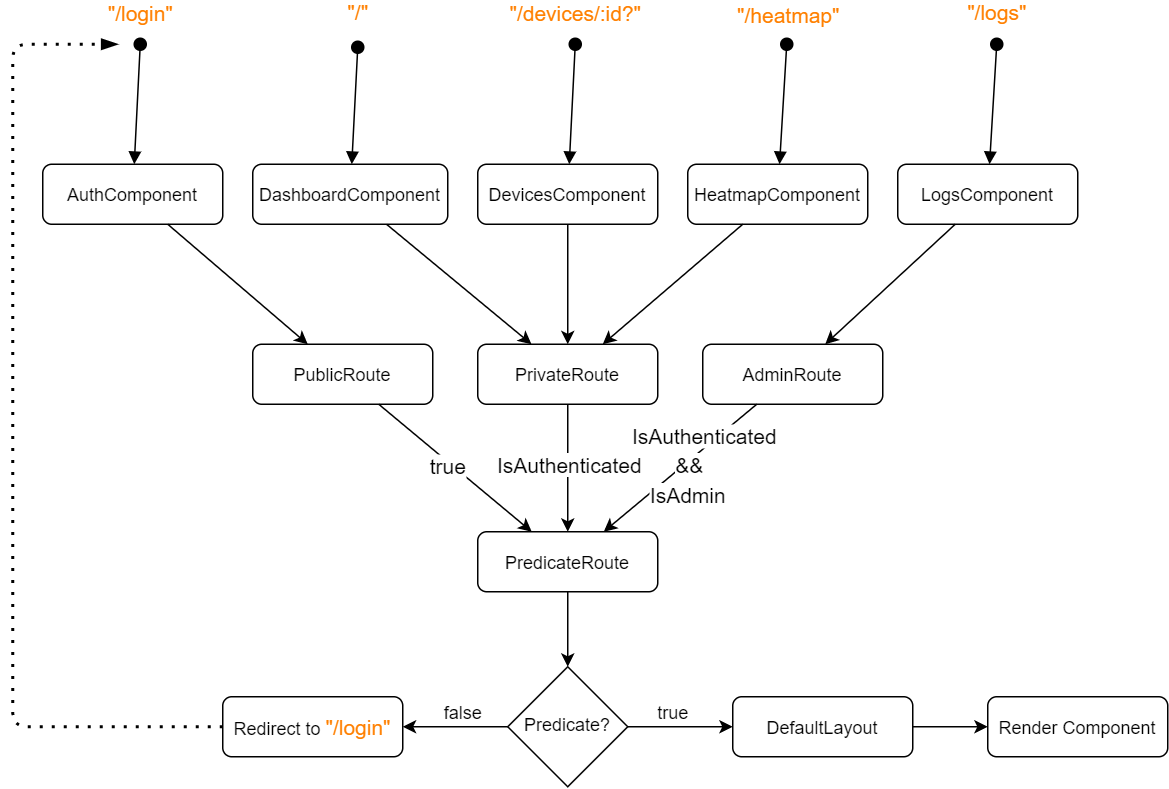
\includegraphics[width=150mm, keepaspectratio]{figures/birdmap-frontend-routes.png}
    \caption{A Birdmap kliensoldalának architektúrája}
    \label{fig:birdmap-frontend-architecture}
\end{figure}

%----------------------------------------------------------------------------
\section{Kommunikáció a szerveroldallal}
%----------------------------------------------------------------------------
A szerveroldallal való kommunikációt rendkívül egyszerűen tudtam implementálni köszönhetően a \ref{subsect:backend-swagger}-as fejezetben bemutatott Swagger oldalnak
és annak, hogy az NSwag Studio-val \cite{nswag-studio} a C\#-on kívül lehet TypeScript\footnotemark klienseket is generálni a leíró fájlból.
Így készültek el a komponensek kommunikációért felelős szolgáltatásai.

\footnotetext{JavaScript-re épített statikus típusdefiníciókat tartalmazó nyelv. JavaScript és TypeScript együtt is használható.}
%----------------------------------------------------------------------------
\section{Komponensek}
%----------------------------------------------------------------------------
Ebben a szakaszban ismertetem az egyes oldalak komponenseit és azok alkomponenseit,
illetve a navigációért felelős fejlécet.
%----------------------------------------------------------------------------
\subsection{Navigáció}
%----------------------------------------------------------------------------
A fejléc két komponensből áll. Az egyik az oldal címe a másik az oldalak linkjeit tartalmazó komponens.
Utóbbit a React \verb+NavLink+ komponenseivel készítettem, melyeknek meg lehet adni, hogy kattintásra hova irányítsa a felhasználót.
Ha a jelenlegi webcím tartalmazza a linknek megadott címet, akkor az aktív státuszba kerül, melyre külön stílus osztályok vonatkoznak.
Ezt használva, az aktív linkeket egy aláhúzással jelölöm. 

\begin{figure}[!ht]
    \centering
    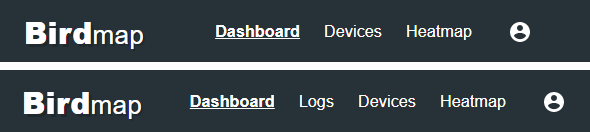
\includegraphics[width=150mm, keepaspectratio]{figures/appbar-user-admin.png}
    \caption{A Birdmap fejléce. Felül a User, alul az Admin felhasználóké}
    \label{fig:birdmap-appbar}
\end{figure}

A fejléc alapértelmezetten része a \verb+DefaultLayout+ komponensnek, így minden oldalon megjelenítésre kerül.

%----------------------------------------------------------------------------
\subsection{Login}
%----------------------------------------------------------------------------
A bejelentkező oldal viszonylag egyszerű. Két szövegdobozt és egy bejelentkező gombot tartalmaz, ahogy az a \ref{fig:birdmap-login}-as ábrán is látszik.

\begin{figure}[!ht]
    \centering
    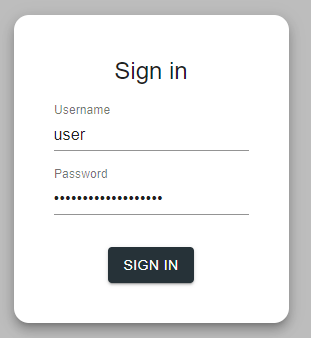
\includegraphics[width=60mm, keepaspectratio]{figures/birdmap-login.png}
    \caption{A Birdmap bejelentkező felülete}
    \label{fig:birdmap-login}
\end{figure}

A generált szerverrel kommunikáló szolgáltatás be van csomagolva egy közösen használt másik szolgáltatásba.
Ennek célja, hogy a bejelentkezés eredményét több komponens is olvashassa, hiszen az alkalmazás felületét alapvetően megkülönbözteti,
egyrészt a bejelentkezés sikeressége, másrészt a bejelentkezett felhasználó jogosultsági köre.

Sikeres bejelentkezés után a szerver elküldi a felhasználó szerepét, illetve a hozzáférési token-t, amelyre a kliens többi szolgáltatásának is szüksége lesz a kommunikációhoz. 
Ezeket az oldal \verb+sessionStorage+-ában\footnotemark tárolom és a becsomagolt szolgáltatáson keresztül elérhetőek.

Kijelentkezni a navigációs fejlécben található profil ikonra való kattintással lehet.

\footnotetext{Webtárhely objektum. Lehetővé teszi a kulcs-érték párok tárolását a böngészőben.}

%----------------------------------------------------------------------------
\subsection{Logs}
%----------------------------------------------------------------------------
Ez az oldal az \verb+Admin+ felhasználó számára lehetővé teszi a szerveren található naplófájlok letöltését \verb+zip+ fájlformátumú archív fájlokban.
Komponense a \ref{fig:birdmap-logs}-es ábrán látható.

\begin{figure}[!ht]
    \centering
    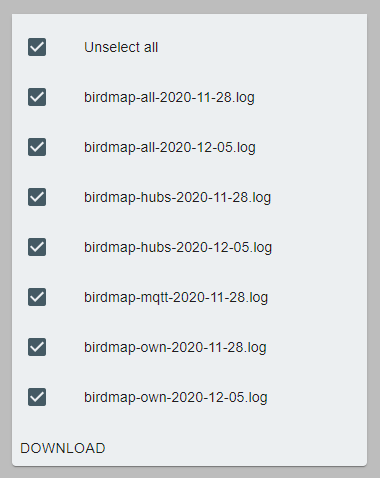
\includegraphics[width=75mm, keepaspectratio]{figures/birdmap-logs.png}
    \caption{A Birdmap naplófájlok letöltésének felülete}
    \label{fig:birdmap-logs}
\end{figure}
%----------------------------------------------------------------------------
\subsection{Eszközállapot- és hangüzenet-kezelő szolgáltatás}
%----------------------------------------------------------------------------
A szakasz további komponenseinek van egy közös ismertetője. Mégpedig, hogy mindegyiknek szüksége van a kihelyezett eszközök adataira
és az azok által publikált hangüzenetekből képzett valószínűségre.
A Reactnek van egy beépített komponense \verb+Context+ \cite{react-context} néven, mellyel különböző komponensek között lehet adatokat megosztani.
Ezt használva készítettem egy \verb+DevicesContextProvider+ osztályt, melynek feladata a szerver eszköz kontrollerével való kommunikáció a megfelelő szolgáltatáson keresztül,
illetve a SignalR csatornákra való feliratkozás. Ezekből az adatokból egy \verb+DevicesContext+ készül, mely a \verb+Provider+ által átadásra kerül annak minden gyerekének.
A \ref{lst:react-switch}-es listában látható, hogy a \verb+DevicesContextProvider+ szülője a \verb+Dashboard+, \verb+Devices+ és \verb+Heatmap+ komponenseknek.

%----------------------------------------------------------------------------
\subsection{Dashboard}
%----------------------------------------------------------------------------
A Dashboard az alkalmazás kezdő oldala. Itt található meg a külső szolgáltatások állapotát vizsgáló komponens,
illetve a kihelyezett eszközök működési folyamatában áttekintést nyújtó diagramok mindegyike.

Az oldal megjelenítésekor elindul egy másodpercenként ismétlődő folyamat,
mely a \verb+DevicesContext+-ből kiolvasott értékekből legenerálja a diagramokon megjelenítendő összes adatot.
Ez azonban az adat mennyiségétől függően akár egy-két másodpercig is eltarthat, ami rendkívül lassúvá és használhatatlanná tenné a felületet.
Ennek elkerülése érdekében az adatfeldolgozó folyamat egyszerre csak egy pár elemet dolgoz fel, mely alfolyamatok között 20 milliszekundum szüneteket iktattam be.
Továbbá hogy a különböző diagramok animációi is zökkenőmentesek legyenek, azok adatai cserélése között is van 300 milliszekundum szünet.
Így valamivel lasabb az adatfeldolgozás, de a felület használható marad.
%----------------------------------------------------------------------------
\subsubsection{Külső szolgáltatások}
%----------------------------------------------------------------------------
Az alkalmazás használatának szempontjából van néhány olyan külső szolgáltatás, melyek elérhetősége hiányában a rendszer működésképtelen.
Ilyen például a Birbnetes klasztere vagy a szerver MQTT szolgáltatása. 
Ezért készítettem el az \ref{fig:dashboard-services-loaded}-ös ábrán látható információs panelt, ahol a szolgáltatások állapotát lehet látni, hogy a felhasználó tudja miért nem működik esetleg az alkalmazás.
A felület megvalósításhoz a Material UI \verb+Accordion+ elemét használtam, ami lényegében egy lenyíló lista. 
Ennek fejlécében a szolgáltatás neve, elérési útvonala és státusza látható. A lenyíló elemben a szolgáltatástól érkezett válasz van megjelenítve. 

\begin{figure}[!ht]
    \centering
    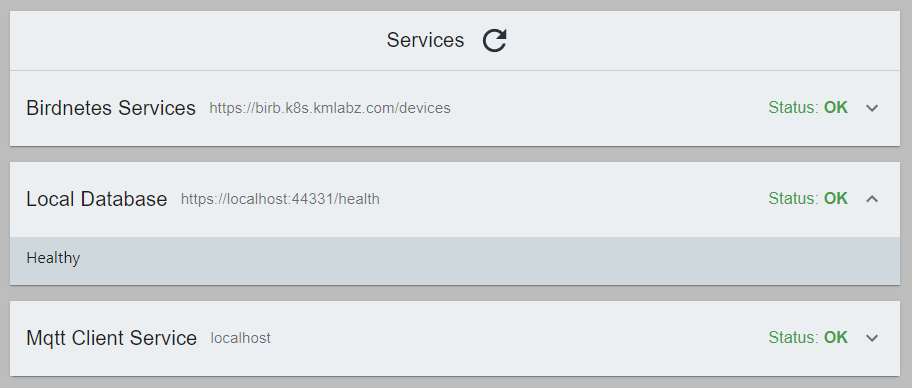
\includegraphics[width=150mm, keepaspectratio]{figures/dashboard-services-loaded.png}
    \caption{Az alkalmazás által használt külső komponensek állapotának megjelenítéséért felelős komponens}
    \label{fig:dashboard-services-loaded}
\end{figure}

Az oldal betöltése vagy a frissítés gomb megnyomása esetén az adatok lekérésre kerülnek a szervertől.
Ez a folyamat akár öt-hat másodpercig is eltarthat, mely közben a felhasználó egy üres listát látna.
Ennek elkerülésére használom a Material UI \verb+Skeleton+ komponensét, 
mely egy megadható méretű töltő csíkkal helyettesíti az \verb+Accordion+-ban található elemeket a \ref{fig:dashboard-services-loading}-os ábrán látható módon.
Azért célszerű ennek a használata, mert így a felhasználónak több információja van arról, hogy a felületen milyen adatok és hol fognak megjelenni.
A felhasználói élmény maximalizálása érdekében a frissítés előtt lekérdezem a szervertől, hogy hány darab szolgáltatás található az adatbázisban 
és annyi darab töltőcsíkos \verb+Accordion+-t jelenítek meg. 

\begin{figure}[!ht]
    \centering
    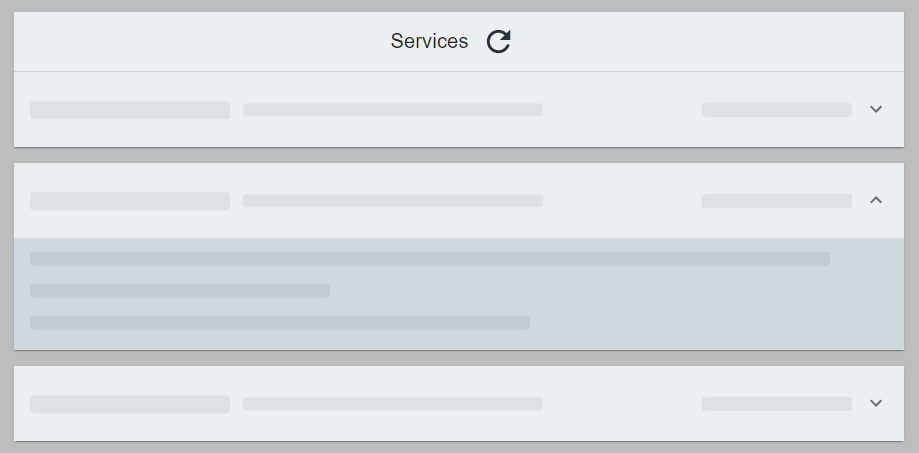
\includegraphics[width=150mm, keepaspectratio]{figures/dashboard-services-loading.png}
    \caption{A Skeletonok alkalmazása a külső szolgáltatások állapotának betöltése közben.}
    \label{fig:dashboard-services-loading}
\end{figure}

%----------------------------------------------------------------------------
\subsubsection{Eszközök és szenzorok állapota}
%----------------------------------------------------------------------------
Ennek a komponensnek a szerepe, hogy áttekintést nyújtson az eszközök és szenzorok állapotáról.
Úgy gondoltam, hogy erre a legcélravezetőbb eszköz a \ref{fig:dashboard-donut}-es ábrán is látható Apexcharts fánk diagramja.
Látható, hogy hány darab eszköz és szenzor van bekapcsolt, kikapcsolt, illetve hibás állapotban.
Az állapotok változása esetén a \verb+DevicesContextProvider+-nek köszönhetően az adatok automatikusan frissülnek.
\begin{figure}[!ht]
    \centering
    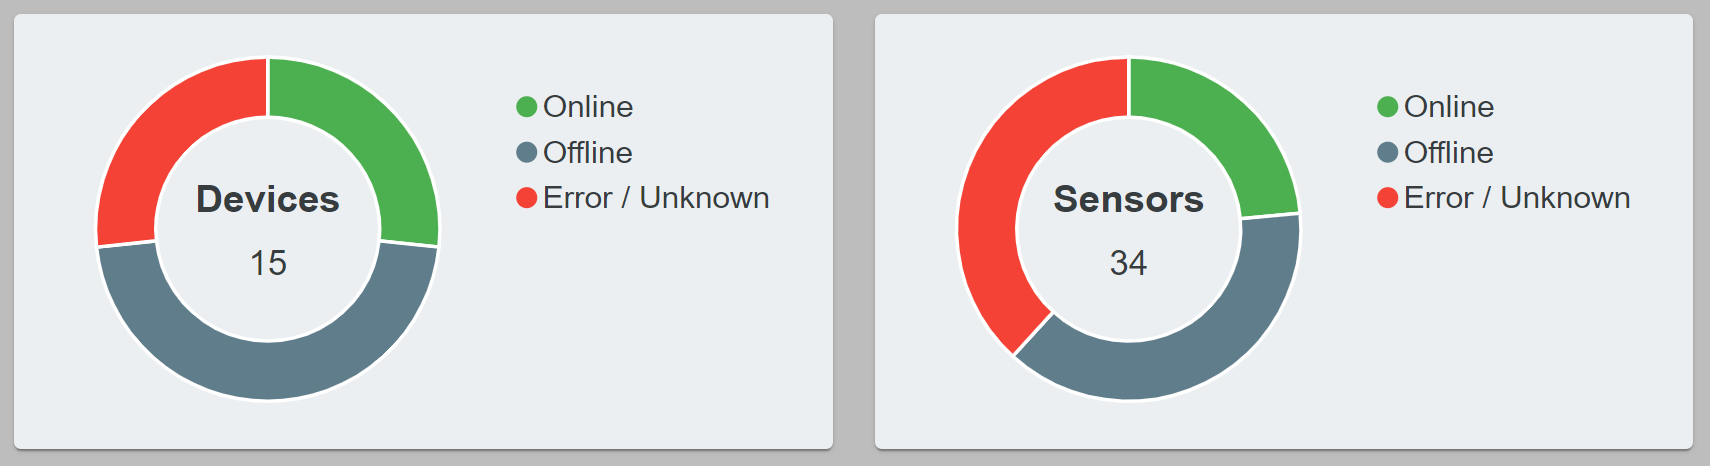
\includegraphics[width=150mm, keepaspectratio]{figures/dashboard-donut-devices.png}
    \caption{A Dashboard eszköz- és szenzor állapotok diagramja}
    \label{fig:dashboard-donut}
\end{figure}
%----------------------------------------------------------------------------
\subsubsection{Hőtérkép diagramok}
%----------------------------------------------------------------------------
Ezekkel a diagramokkal az a célom, hogy az eszközök által küldött észleléseket időrendben vizualizáljam.
Megvalósításukhoz az Apexcharts Heatmap típusú diagramját használtam.
A \ref{fig:dashboard-heatmap-second}-as ábrán látható diagram az elmúlt egy percben küldött, másodpercenként a legnagyobb, hangüzenetekből képzett valószínűségeket ábrázolja.
A \ref{fig:dashboard-heatmap-minute}-es ábrán látható diagram pedig az elmúlt egy órában percenként a legnagyobbakat.
\begin{figure}[!ht]
    \centering
    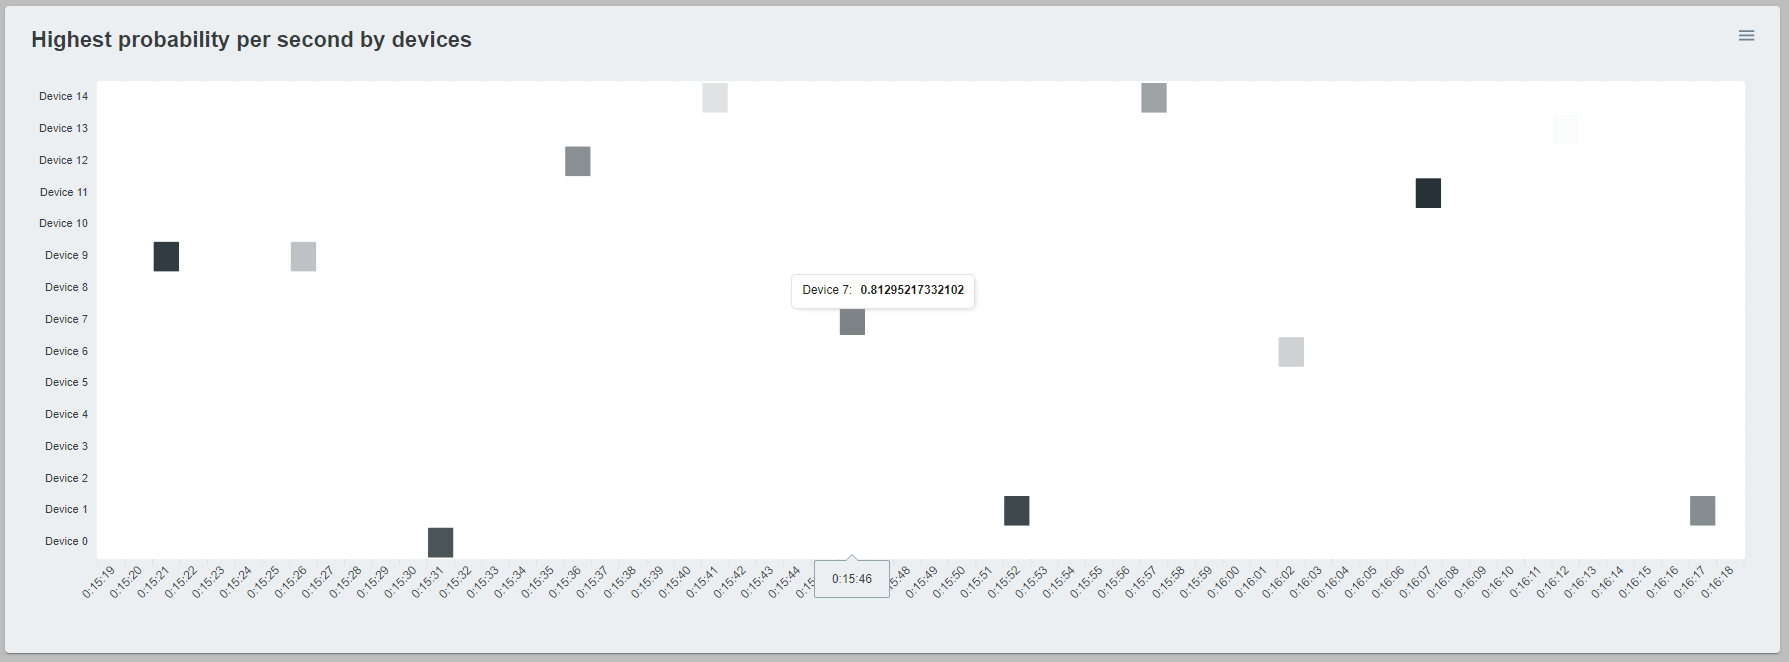
\includegraphics[width=150mm, keepaspectratio]{figures/second-heatmap.png}
    \caption{Másodperc alapú hőtérképes diagram}
    \label{fig:dashboard-heatmap-second}
\end{figure}
\begin{figure}[!ht]
    \centering
    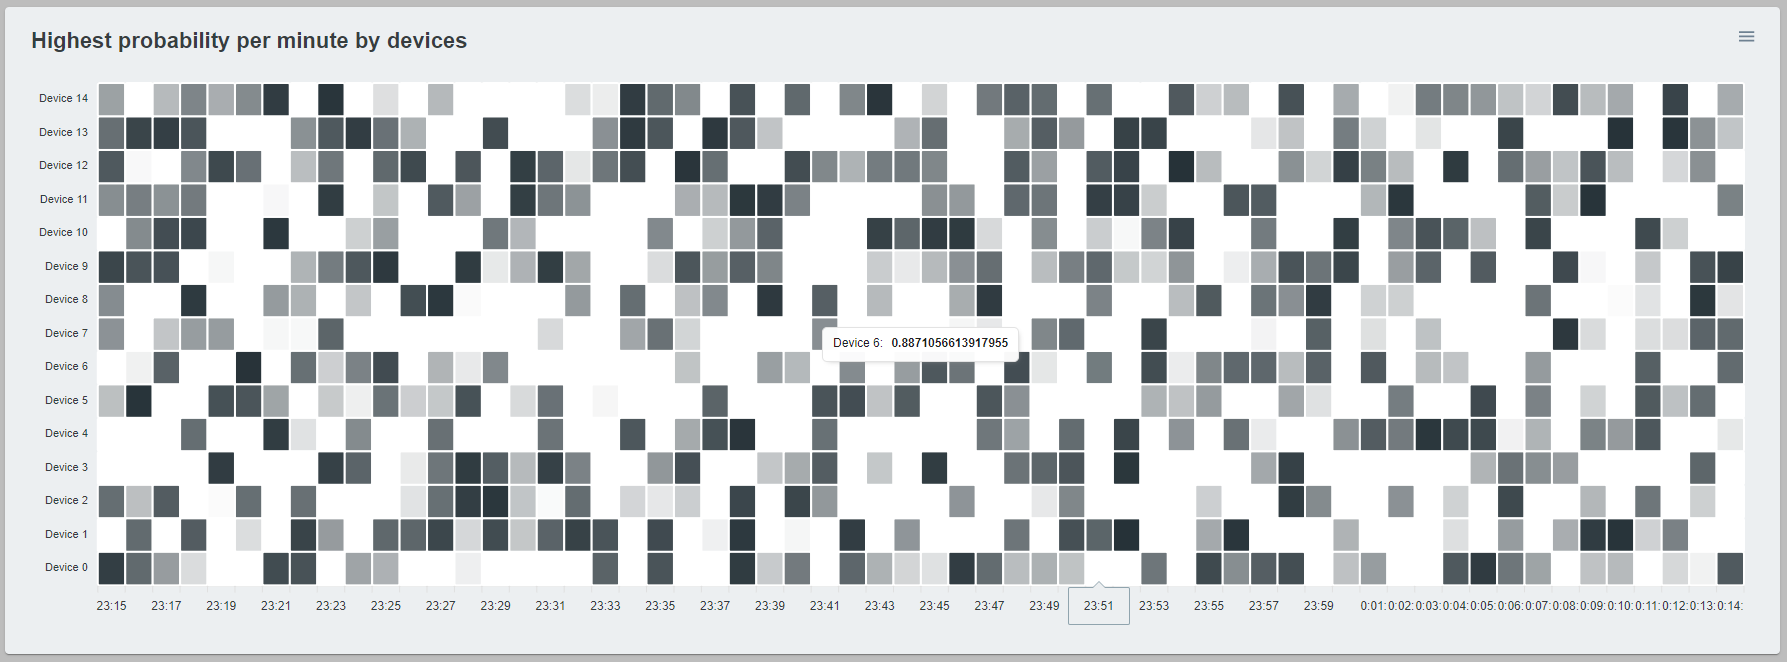
\includegraphics[width=150mm, keepaspectratio]{figures/minute-heatmap.png}
    \caption{Perc alapú hőtérképes diagram}
    \label{fig:dashboard-heatmap-minute}
\end{figure}

A függőleges tengelyen a rendszer eszközei vannak dinamikusan megjelenítve.
A vízszintes tengelyen pedig az említett időtartományok.
A diagramokon látható négyzetek a valószínűség nagyságától függően sötétebbek vagy világosabbak.
\newpage
%----------------------------------------------------------------------------
\subsubsection{Riasztás számláló}
%----------------------------------------------------------------------------
Ez egy egyszerű oszlopdiagram, mely aggregálja az egyes eszközök által küldött hangüzeneteket 0.5 valószínűség felett a \ref{fig:dashboard-devices-column}-es ábrán látható módon.
Segítségével megvizsgálható, hogy mely eszközök riasztanak a legtöbbet a legnagyobb valószínűséggel.
\begin{figure}[!ht]
    \centering
    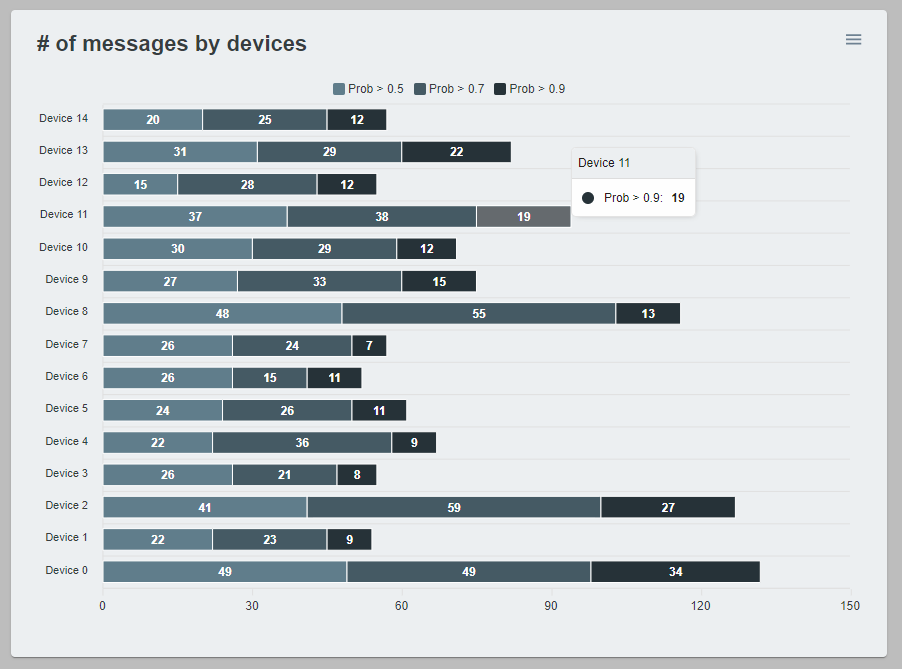
\includegraphics[width=150mm, keepaspectratio]{figures/dashboard-column-devices.png}
    \caption{Eszközönkénti riasztásokat számláló diagram}
    \label{fig:dashboard-devices-column}
\end{figure}

Az egyes oszlopok három részre vannak bontva az üzenetek öt tized, hét tized és kilenc tized fölötti valószínűsége szerint. 
\newpage
%----------------------------------------------------------------------------
\subsubsection{Üzenetek gyakorisága}
%----------------------------------------------------------------------------
Az oldalon található utolsó diagram egy vonal diagram, melynek célja, hogy ábrázolja a rendszer által küldött üzenetek számát másodpercenként.
A \ref{fig:dashboard-messages-line}-es ábrán látható a komponens.
A vízszintes tengelyen a legelső érték az alkalmazás által először észlelt üzenet időpontja.
Az utolsó érték a legutoljára észlelt időpontja.
A függőleges tengelyen az adott másodpercben érkező üzenetek száma van ábrázolva.
Az előzőkkel ellentétben itt az adatok nincsennek szűrve a hangüzenet valószínűsége alapján,
tehát a rendszer által küldött összes üzenet látható.
\begin{figure}[!ht]
    \centering
    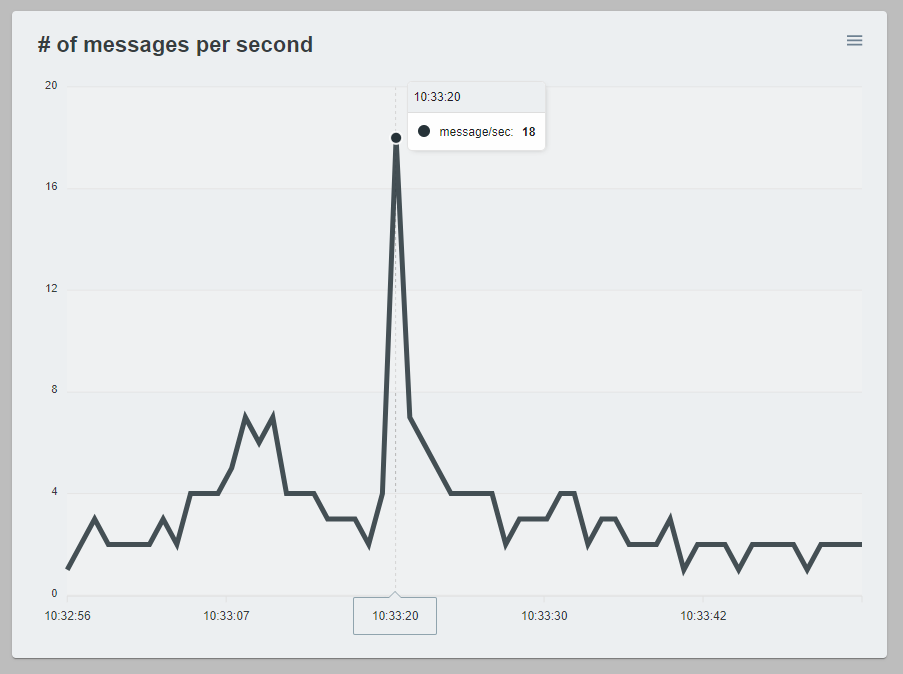
\includegraphics[width=150mm, keepaspectratio]{figures/dashboard-line-messages.png}
    \caption{A másodpercenként érkező üzenetek számát ábrázoló diagram.}
    \label{fig:dashboard-messages-line}
\end{figure}
\newpage
%----------------------------------------------------------------------------
\subsection{Devices}
%----------------------------------------------------------------------------
Ez az oldal lehetővé teszi a felhasználók számára az eszközök állapotának áttekintését, \verb+Admin+ felhasználók számára azok menedzselését is.
Az eszközök dinamikusan jelennek meg a \verb+DevicesContextProvider+ adatai alapján, melyek megjelenítésére a Material UI \verb+Accrordion+ komponensét használom.
Ennek fejlécében az eszköz neve, egyedi azonosítója és státusza található. A lenyíló részben pedig az eszköz által használt szenzorok neve, azonosítója és státusza.
\verb+Admin+ felhasználók számára a felület két fajta gombbal bővül, melyekkel be és ki lehet kapcsolni az egyes eszközöket, szenzorokat.
Az \verb+Accordion+-ok felett található egy külön panel, mellyel egyszerre lehet kezelni az összes eszközt és azok szenzorjait.
A Devices oldal felülete a \ref{fig:frontend-devices}-es ábrán,
az \verb+Admin+ felhasználók számára nyújtott plusz funkciók a \ref{fig:frontend-devices-admin}-as ábrán láthatók.
\begin{figure}[!ht]
    \centering
    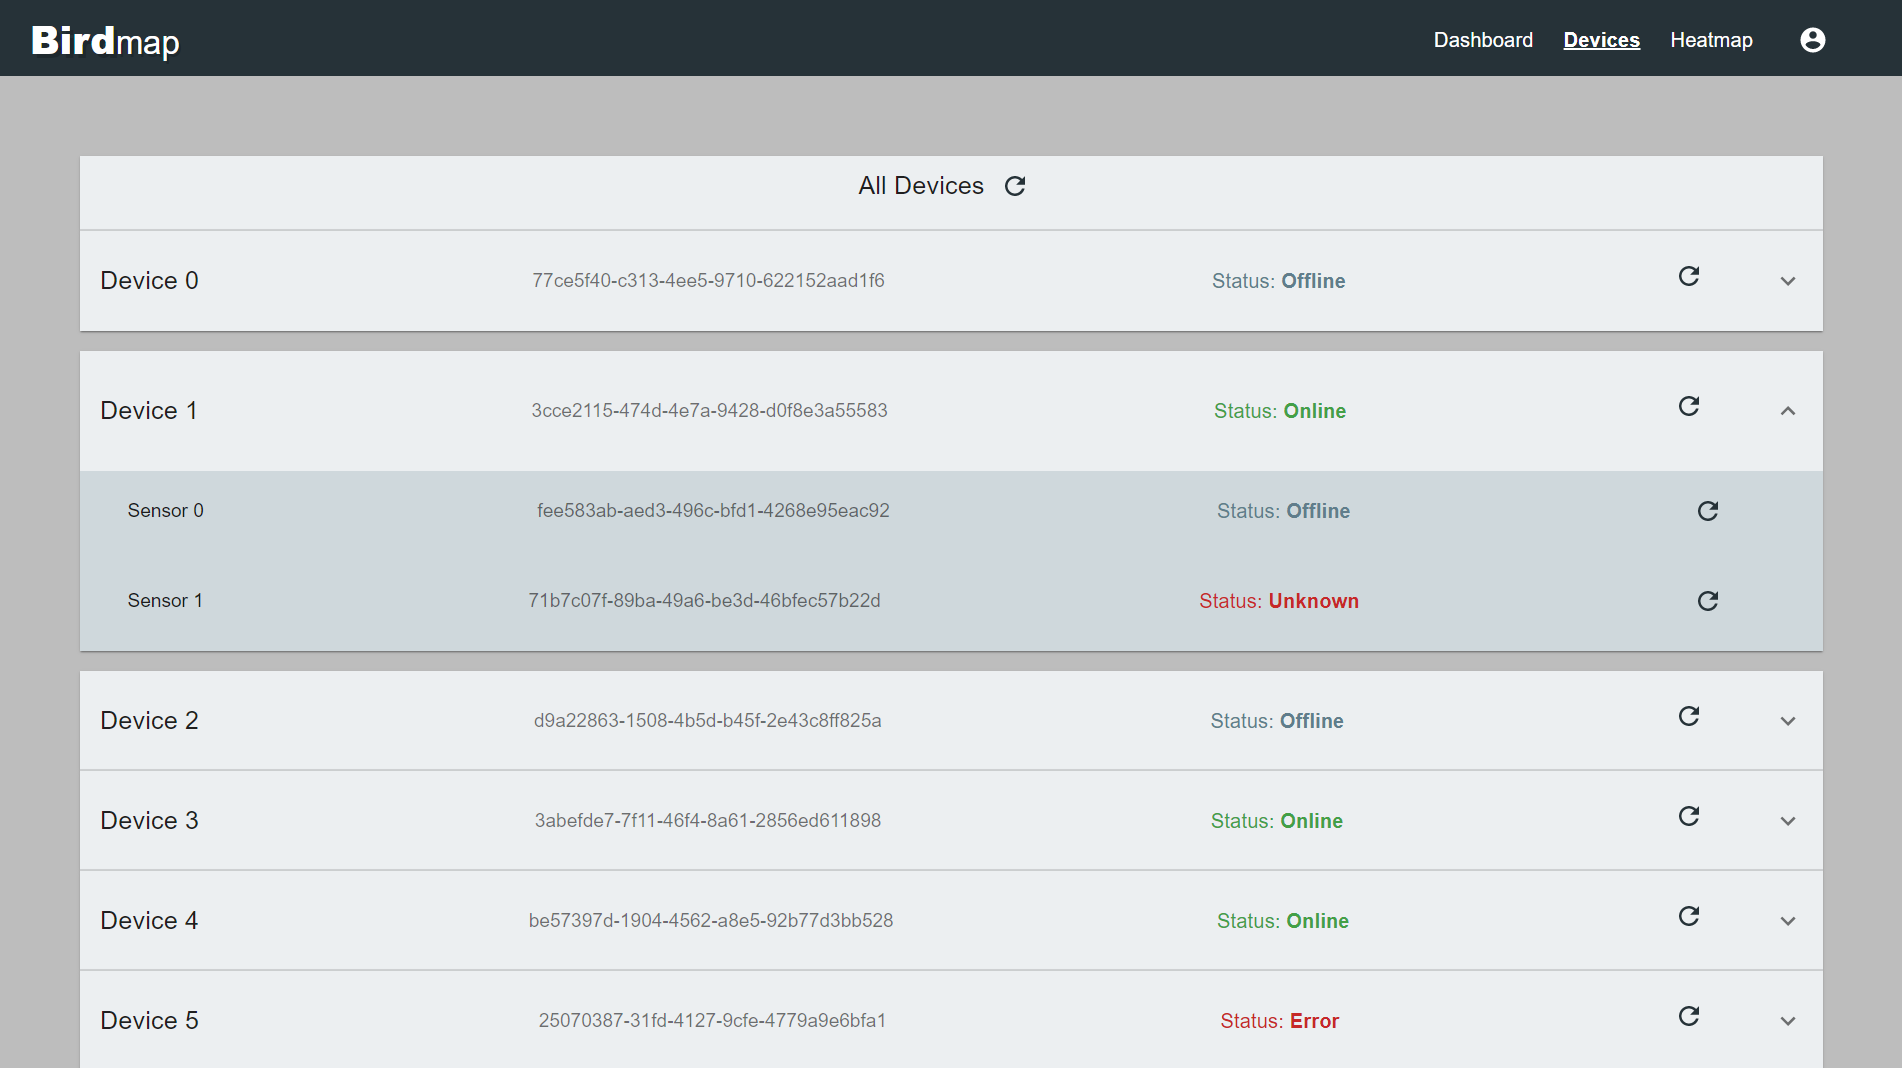
\includegraphics[width=150mm, keepaspectratio]{figures/devices.png}
    \caption{A Devices oldal felülete.}
    \label{fig:frontend-devices}
\end{figure}
\begin{figure}[!ht]
    \centering
    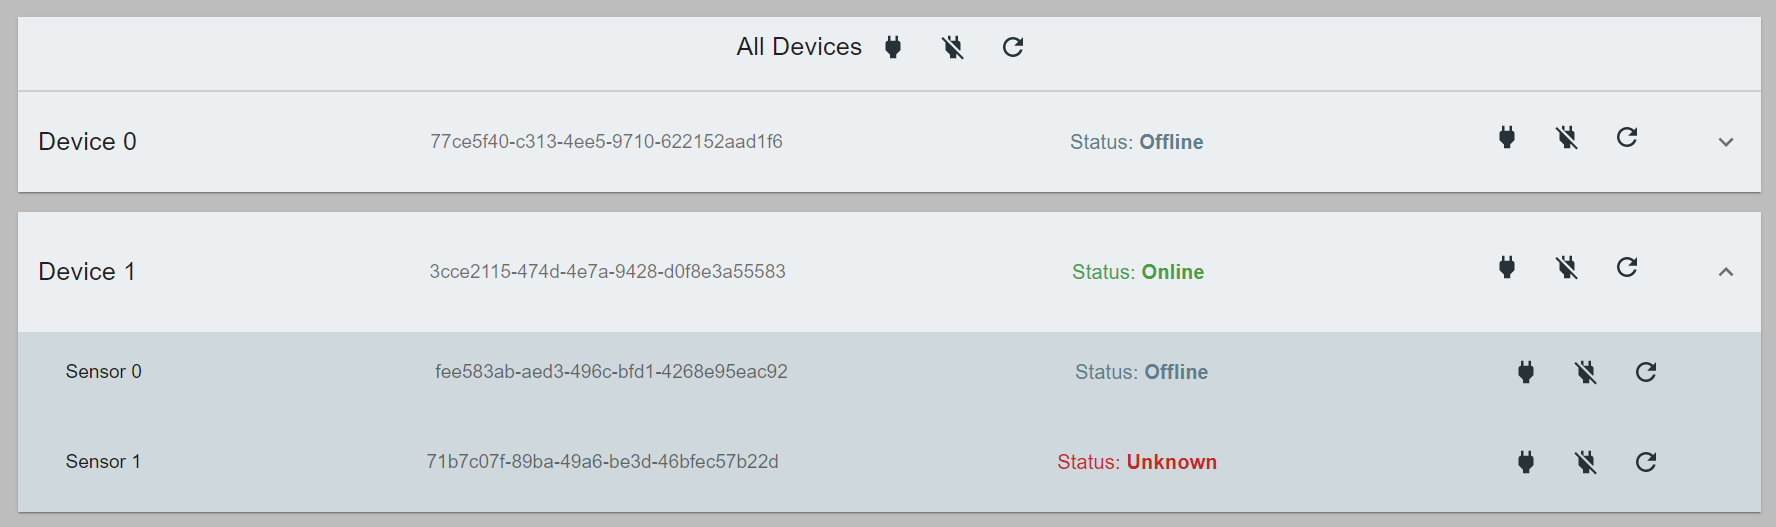
\includegraphics[width=150mm, keepaspectratio]{figures/devices-admin.png}
    \caption{Az Admin felhasználók számára elérhető plusz funkciók.}
    \label{fig:frontend-devices-admin}
\end{figure}
%----------------------------------------------------------------------------
\subsection{Heatmap}
%----------------------------------------------------------------------------
Az alkalmazással szemben az egyik legfontosabb követelmény a hőtérképes vizualizáció volt,
mely ezen az oldalon található. A Google Maps API segítségével megjelenítek egy térképet a felületen,
majd erre kerül a hőtérképes réteg. A térképre szélességi és hosszúsági körök alapján lehet rajzolni.
Ezt használva megjelenítem a rendszer összes eszközét azok koordinátái szerint.
A kék színű ikonok jelölik a bekapcsolt állapotban lévő, a sárga a kikapcsolt állapotban lévő,
a piros pedig a hibás állapotban lévő eszközöket.
Ha a felhasználó az egerét az ikonok fölé helyezi, megjelenik egy szövegdoboz, melyben az eszköz azonosítója és státusza látható. 
Az ikonra kattintva a felhasználó a Devices oldalra kerül, ahol megnyílik a kattintott eszköz \verb+Accordion+-ja.

A \verb+DevicesContext+ tartalmazza az eszközök által küldött üzenetek adatait,
melyeknek a 0.5 valószínűségtől nagyobb részhalmazát a hőtérkép által kezelhető adatokká konvertálok.
Egyrészt szükség van az előbb is említett földrajzi koordinátákra, melyeket az üzenetek eszköz azonosítója alapján határozok meg.
Másrészt szükség van egy súly értékre, mely a pont színezésének pirosságát határozza meg.
Ezt az értéket az üzenetek valószínűség értékével tettem egyenlővé.
Minél több magasabb valószínűségű riasztás érkezik egy adott eszköztől, a körülötte lévő terület annál pirosabb lesz.

A \ref{fig:frontend-heatmap}-ös ábra mutatja a térkép működését miközben 4 eszköz is seregélyeket észelt.

\begin{figure}[!ht]
    \centering
    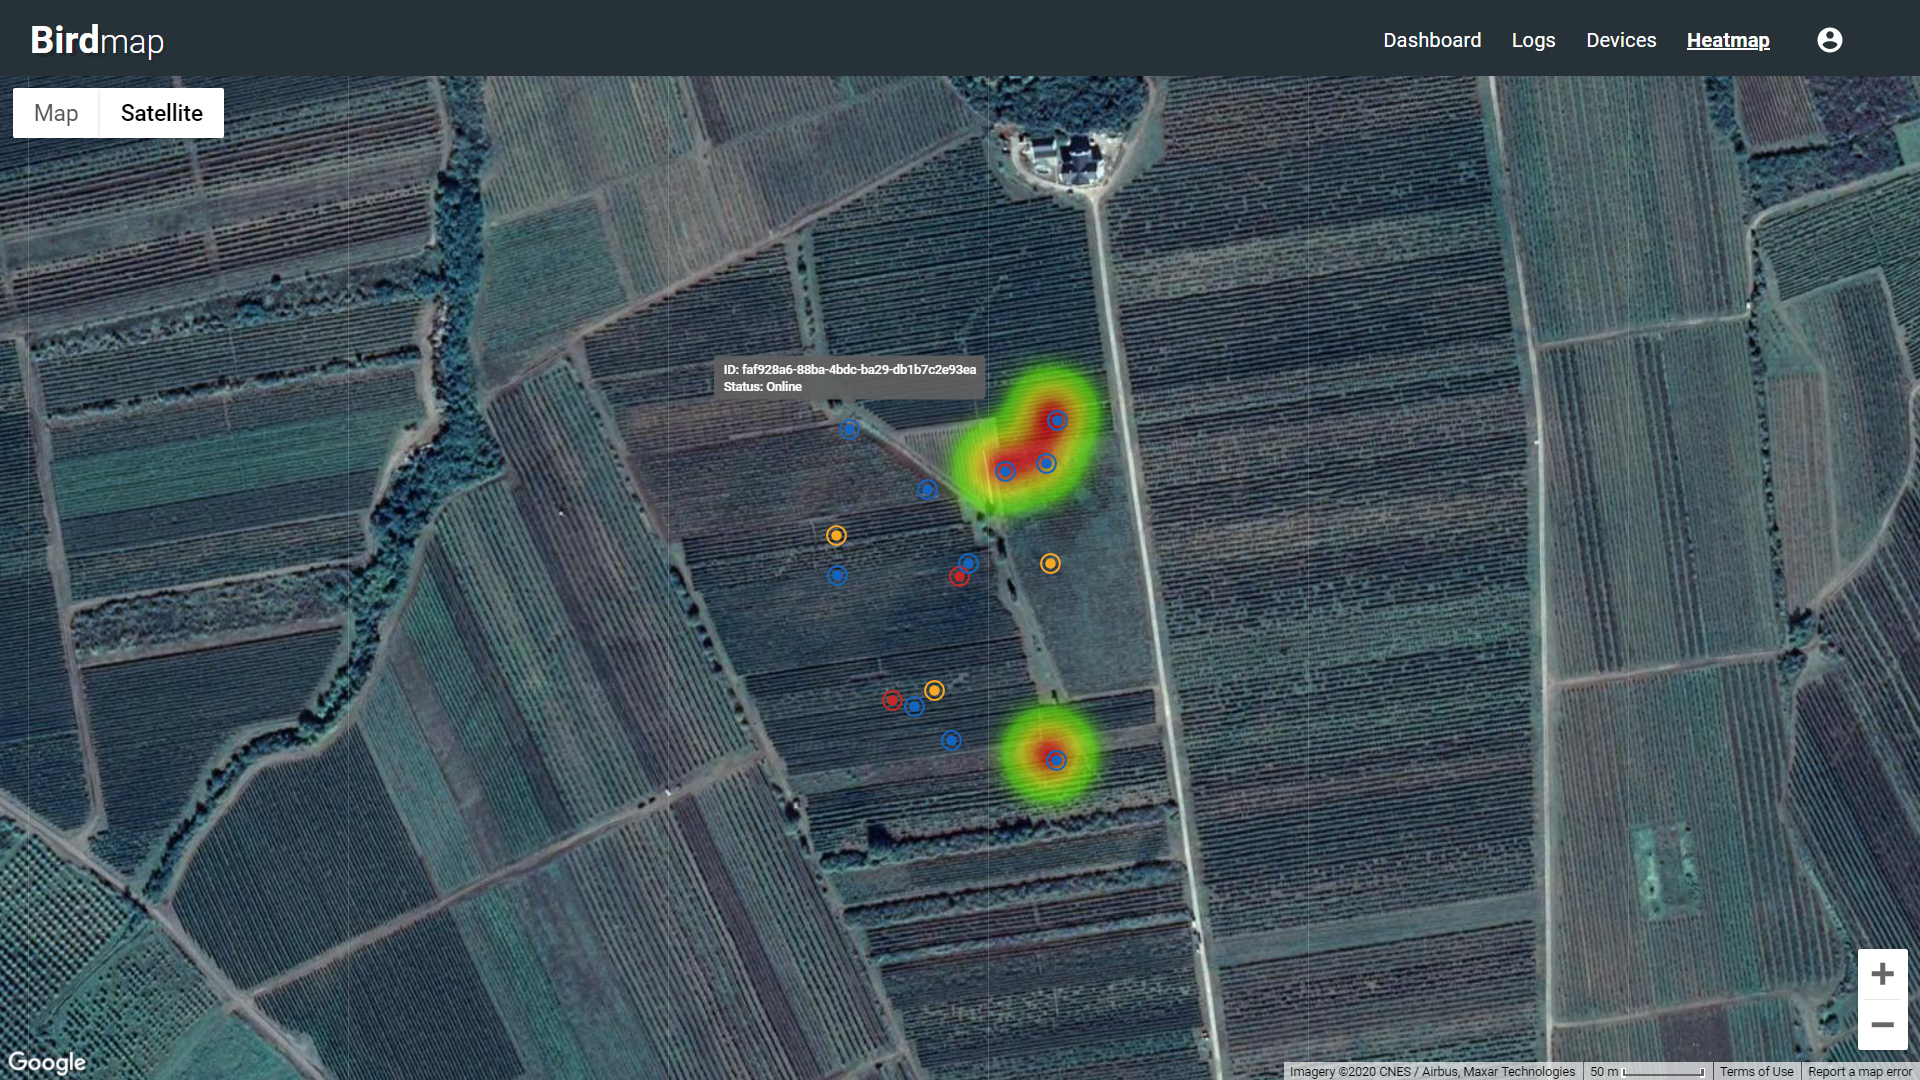
\includegraphics[width=150mm, keepaspectratio]{figures/heatmap.png}
    \caption{A Heatmap oldal felülete.}
    \label{fig:frontend-heatmap}
\end{figure}
%----------------------------------------------------------------------------
\chapter{Tesztkörnyezet}
\label{chapt:birdmap-test}
%----------------------------------------------------------------------------
Az alkalmazásom fejlesztésének megkönnyítése érdekében nagy hangsúlyt fektettem a tesztelhetőségre.
Helyettesíteni akartam az éles rendszer komponenseivel való kommunikációt,
hogy abban az esetben is folyni tudjon a fejlesztés, ha a rendszer épp nem elérhető.
Ezen kívül hasznos, ha az alkalmazás által feldolgozott adatok személyre szabhatóak,
hiszen sokszor olyan problémákra lehet így fényt deríteni, amelyek nem vagy csak jóval később jönnének elő az éles rendszer használata során.

A tesztelhetőség megvalósításához három szoftver komponenst kell helyettesítenem,
melyeket az alábbi szekciókban ismertetek.
%----------------------------------------------------------------------------
\section{Helyettesítő szolgáltatások}
%----------------------------------------------------------------------------
Az alkalmazásom szerver oldali szolgáltatásai a Birbnetes Command and Control (a kódban Device) és Input Service-ekkel azok OpenAPI leíróiból generált interfészein keresztül kommunikál.
Ezen intefészek mögé bármilyen implementáció regisztrálható, mely helyettesíti az éles rendszer működését.

Készítettem egy osztályt \verb+DummyDeviceAndInputService+ néven, mely a szerver indulásakor mű eszközadatokat generál egy lokális változóval állítható darabszámban,
majd ezeket egy belső listában tárolja. Az eszközök státuszát és koordinátáit egy véletlenszám generátor segítségével határozom meg.
Az osztály implementálja a Device Service interfészét, melynek metódusai az imént említett mű eszközlista elemeivel dolgoznak,
azok státuszát olvassák és módosítják.
Illetve implementálja az Input Service interfészét, 
melynek metódusa bármilyen paraméterből kapott egyedi azonosító esetén visszaad egy véletlenszerűen kiválasztott bekapcsolt státuszú eszközt a listából.

Az alkalmazás által regisztrált és ezáltal használt intefész implementációi a konfigurációs fájl egy logikai értéke alapján cserélhető az éles és a helyettesítő között,
a \ref{lst:dummy-service-registration}-es listában látható módon.
\newpage
\begin{lstlisting}[style=csharp, caption=A helyettesítő és az éles szolgáltatások regisztrálásának logikája, label=lst:dummy-service-registration]
    if (configuration.GetValue<bool>("UseDummyServices"))
    {
        services.AddTransient<IInputService, DummyDeviceAndInputService>();
        services.AddTransient<IDeviceService, DummyDeviceAndInputService>();
    }
    else
    {
        services.AddTransient<IInputService, LiveInputService>();
        services.AddTransient<IDeviceService, LiveDeviceService>();
    }
\end{lstlisting}


%----------------------------------------------------------------------------
\section{MQTT tesztalkalmazás}
%----------------------------------------------------------------------------
Az MQTT.NET szoftvercsomag github oldalán található néhány példa a csomag használatára \cite{mqttnet-examples}.
Ezek között találtam Sepp Penner MQTTnet.TestApp.WinForm \cite{mqttnet-winforms} projektjét, 
mely egy Windows Forms applikáció az említett szoftvercsomag által nyújtott funkcionalitások tesztelésére.
Indítható vele MQTT szerver, feliratkozó kliens és publikáló kliens is.
Ezek meglétével az alkalmazás képes az üzenetek manuális publikálására egy a felületen beállítható témában.
Én azonban szerettem volna az üzeneteket automatikusan bizonyos időközönként küldeni,
ezért átalakítottam az alkalmazást az igényeimnek megfelelően a \ref{fig:mqtt-tester}-es ábrán látható módon.
Elhelyeztem a fejlületen egy csúszkát, mellyel az üzenet küldés intervalluma állítható, illetve két új gombot,
melyekkel az üzenet küldő időzítő indítható és megállítható.
Az alkalmazás képes üzenetek adatainak generálására, mellyel az AI Service által publikált üzenetek modelljeivel azonos adatokat generálok.
\begin{figure}[!ht]
    \centering
    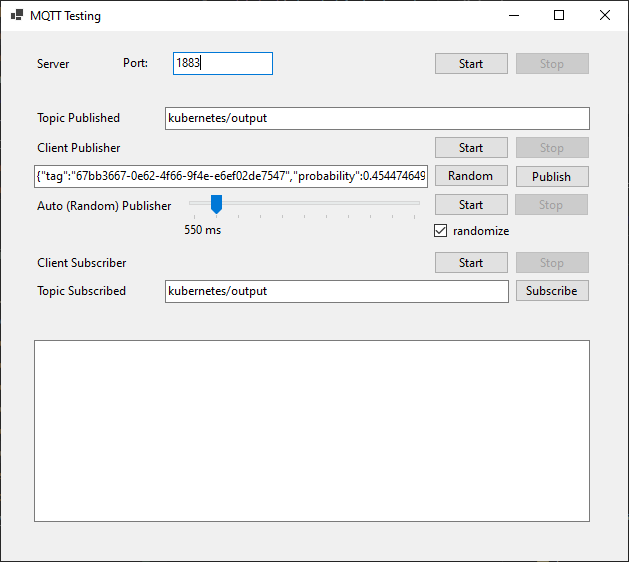
\includegraphics[width=150mm, keepaspectratio]{figures/MQTT-Tester.png}
    \caption{Az MQTT kommunikációt tesztelő alkalmazás felületének egy része}
    \label{fig:mqtt-tester}
\end{figure}

%----------------------------------------------------------------------------
\chapter{Kubernetes}
\label{chapt:birdnetes-kubernetes}
%----------------------------------------------------------------------------
%----------------------------------------------------------------------------
\chapter{Értékelés}
\label{chapt:summary}
%----------------------------------------------------------------------------
Úgy gondolom, hogy az alkalmazásom elérte a célját.
Egy használható felületet nyújt a Birbnetes mikroszolgáltatás rendszere működésének vizualizálására.
A fejlesztés közben jelentős figyelmet fordítottam arra, hogy az alkalmazás felületi és kód komponensei között is
minimalizáltak legyenek a függőségek, így a rendszerben történő változások esetén azok könnyen cserélhetőek, bővíthetőek.
%----------------------------------------------------------------------------
\section{Továbbfejlesztési lehetőségek}
%----------------------------------------------------------------------------
Az kliens oldalon történő diagramok adatainak generálása hamar túl nagy falatnak bizonyult.
A bevetett optimalizációk ellenére sem lett hatványozottan gyorsabb a felület.
Így az első és legfontosabb továbbfejlesztési teendő az adatok szerveroldalon történő generálása lenne.

A Logs oldal jelenleg csak a szerveroldalon készült napló fájlokat tartalmazza.
Hasznos lenne, ha az egyes mikroszolgáltatások naplófájljai is letölthetőek lennének.

Ezen kívül előnyös lenne a rendszer belső működését vizualizáló komponensek alkalmazása is, 
ahol lehetne látni az egyes mikroszoltáltatásokra vonatkozó különböző metrikákat például az adatfeldolgozási időt vagy a beérkezett kérések számát. 

% List of Figures, Tables
%~~~~~~~~~~~~~~~~~~~~~~~~~~~~~~~~~~~~~~~~~~~~~~~~~~~~~~~~~~~~~~~~~~~~~~~~~~~~~~~~~~~~~~
%\listoffigures\addcontentsline{toc}{chapter}{\listfigurename}
%\listoftables\addcontentsline{toc}{chapter}{\listtablename}


% Bibliography
%~~~~~~~~~~~~~~~~~~~~~~~~~~~~~~~~~~~~~~~~~~~~~~~~~~~~~~~~~~~~~~~~~~~~~~~~~~~~~~~~~~~~~~
\addcontentsline{toc}{chapter}{\bibname}
\bibliography{bib/mybib}


% Appendix
%~~~~~~~~~~~~~~~~~~~~~~~~~~~~~~~~~~~~~~~~~~~~~~~~~~~~~~~~~~~~~~~~~~~~~~~~~~~~~~~~~~~~~~
%%----------------------------------------------------------------------------
\appendix
%----------------------------------------------------------------------------
\chapter*{\fuggelek}\addcontentsline{toc}{chapter}{\fuggelek}
\setcounter{chapter}{\appendixnumber}
%\setcounter{equation}{0} % a fofejezet-szamlalo az angol ABC 6. betuje (F) lesz
\numberwithin{equation}{section}
\numberwithin{figure}{section}
\numberwithin{lstlisting}{section}
%\numberwithin{tabular}{section}

%----------------------------------------------------------------------------
\section{A Docker image készítéséhez használt fájlok}
%----------------------------------------------------------------------------
\begin{lstlisting}[style=dockerfile, caption=A Dockerfile tartalma, label=lst:dockerfile]
    FROM mcr.microsoft.com/dotnet/aspnet:5.0 AS base
    WORKDIR /app
    RUN apt-get update && apt-get install -y curl
    RUN curl -sL https://deb.nodesource.com/setup_12.x | bash -
    RUN apt-get update && apt-get install -y nodejs

    FROM mcr.microsoft.com/dotnet/sdk:5.0 AS build
    RUN apt-get update && apt-get install -y curl
    RUN curl -sL https://deb.nodesource.com/setup_12.x | bash -
    RUN apt-get update && apt-get install -y nodejs
    WORKDIR /src
    COPY ["Birdmap.API/Birdmap.API.csproj", "Birdmap.API/"]
    COPY ["Birdmap.BLL/Birdmap.BLL.csproj", "Birdmap.BLL/"]
    COPY ["Birdmap.Common/Birdmap.Common.csproj", "Birdmap.Common/"]
    COPY ["Birdmap.DAL/Birdmap.DAL.csproj", "Birdmap.DAL/"]
    RUN dotnet restore "Birdmap.API/Birdmap.API.csproj"
    COPY . .
    WORKDIR "/src/Birdmap.API"
    RUN dotnet build "Birdmap.API.csproj" -c Release -o /app/build

    FROM build AS publish
    RUN dotnet publish "Birdmap.API.csproj" -c Release -o /app/publish

    FROM base AS final
    WORKDIR /app
    COPY --from=publish /app/publish .
    ENTRYPOINT ["dotnet", "Birdmap.API.dll"]
\end{lstlisting}

\begin{lstlisting}[style=docker-compose, caption=A docker-compose.yml fájl tartalma, label=lst:docker-compose]
    version: '3.4'

    services:
        db:
            image: "mcr.microsoft.com/mssql/server:2019-latest"
            environment:
              - ACCEPT_EULA=Y
              - SA_PASSWORD=RPSsql12345
    
        birdmap.api:
            image: ${DOCKER_REGISTRY-}birdmapapi
            ports:
                - "8000:80"
                - "8001:443"
            volumes:
                - ${APPDATA}/Microsoft/UserSecrets:/root/.microsoft/usersecrets:ro
                - ${APPDATA}/ASP.NET/Https:/root/.aspnet/https:ro
            build:
                context: .
                dockerfile: Birdmap.API/Dockerfile
            depends_on:
                - db
            environment:
                ...
                - Birdmap_LocalDbConnectionString=Data Source=db;Initial Catalog=birdmap;User=sa;Password=RPSsql12345
                - Birdmap_Defaults__Users__0__Name=admin
                - Birdmap_Defaults__Users__0__Password=pass
                - Birdmap_Defaults__Users__0__Role=Admin
                - Birdmap_Defaults__Users__1__Name=user
                - Birdmap_Defaults__Users__1__Password=pass
                - Birdmap_Defaults__Users__1__Role=User
                - Birdmap_Defaults__Services__Local-Database=https://localhost:8001/health
                - Birdmap_Defaults__Services__KMLabz-Service=https://birb.k8s.kmlabz.com/devices
                - Birdmap_UseDummyServices=true
                - Birdmap_ServicesBaseUrl=https://birb.k8s.kmlabz.com/
                - Birdmap_Mqtt__BrokerHostSettings__Host=localhost
                - Birdmap_Mqtt__BrokerHostSettings__Port=1883
                - Birdmap_Mqtt__ClientSettings__Id=ASP.NET Core client
                - Birdmap_Mqtt__ClientSettings__Username=username
                - Birdmap_Mqtt__ClientSettings__Password=password
                - Birdmap_Mqtt__ClientSettings__Topic=devices/output
\end{lstlisting}

%\label{page:last}
\end{document}
